\chapter{Experiments}
%VOLENDO QUI METTERE FOTO DEL DRONE REALE
In this chapter we present the implementation details of the experiments,
the values of the employed parameters and the results obtained from the simulations.
In particular, the parameters relative to the UAVs physical
characteristics used in the simulations are from 
the real Dragonfly IV drone \cite{drone}, these values are
summarized in Table\ref{tab:drone_parameters}.
\begin{table}[h!]
\centering
\caption{\textbf{Drone Physical Parameters}}
\begin{tabular}{c c c c}
\hline\hline
\textbf{Symbol}  & \textbf{Value}       & \textbf{Unit}         & \textbf{Description} \\ \hline\hline
\(m\)           & \(0.4\)              & \(\text{kg}\)          & Total mass of the drone \\
\(J_x\)         & \(3.8278 \times 10^{-3}\) & \(\text{kg}\cdot\text{m}^2\) & Moment of inertia about $x$-axis \\
\(J_y\)         & \(3.8278 \times 10^{-3}\) & \(\text{kg}\cdot\text{m}^2\) & Moment of inertia about $y$-axis \\
\(J_z\)         & \(7.1345 \times 10^{-3}\) & \(\text{kg}\cdot\text{m}^2\) & Moment of inertia about $z$-axis \\
\(l\)           & \(0.205\)            & \(\text{m}\)           & Distance from center to rotor \\
\(c_t\)         & \(6.354 \times 10^{-4}\) & --                     & Coefficient for thrust generation \\
\(c_d\)         & \(0.048\)            & --                     & Coefficient for torque generation \\
\hline\hline
\end{tabular}
\label{tab:drone_parameters}
\end{table}

\section{Implementation}
The implementation of this work is done in \textit{Matlab} and it
is structured into multiple sections and files, to increase the modularity and 
readability of the code while simplifying the debugging process at the same time. 
The entire code is divided into the following categories:
\begin{itemize}
    \item A folder containing the \textbf{RLS} algorithm in the case where the sources
    do not influence one another;
    \item A folder containing the complete \textbf{PSO} algorithm integrated with 
    the PID control (the main focus of our work);
    \item A file with the complete \textbf{NSS} analysis of rotational invariance
    and symmetry properties;
    \item A file with the \textbf{PID} control applied to tracking the initial trajectory
    the drones follow for setup.
\end{itemize}
Th latter contains the same controller and model functions of the \texttt{Controller}
class of the PSO algorithm. The only difference consists in the desired velocities and positions, 
which are given by a predefined trajectory and by the PSO algorithm
respectively.

\noindent\\
In both the last two experiments (trajectory tracking and PSO with
control) the controller gains are chosen with values as
described in Table~\ref{tab:control_gains}:
\begin{table}[h!]
\centering
\caption{\textbf{Control Gains for Position and Attitude Control}}
\begin{tabular}{c c | c c | c}
\hline\hline
\multicolumn{2}{c|}{\textbf{Proportional Gain (\(k_p\))}} & \multicolumn{2}{c|}{\textbf{Derivative Gain (\(k_d\))}} & \textbf{Control Type} \\ \hline
\textbf{Symbol}       & \textbf{Value}       & \textbf{Symbol}       & \textbf{Value}       &                      \\ \hline\hline
\(k_{xp}\)           & 0.1                 & \(k_{xd}\)           & 0.5                 & Position \(x\)       \\
\(k_{yp}\)           & 0.1                 & \(k_{yd}\)           & 0.54                & Position \(y\)       \\
\(k_{zp}\)           & 1.0                 & \(k_{zd}\)           & 2.5                 & Position \(z\)       \\ \hline
\(k_{p\phi}\)        & 2.0                 & \(k_{d\phi}\)       & 2.5                 & Roll \(\phi\)        \\
\(k_{p\theta}\)      & 2.0                 & \(k_{d\theta}\)     & 2.5                 & Pitch \(\theta\)     \\
\(k_{p\psi}\)        & 2.0                 & \(k_{d\psi}\)       & 4.0                 & Yaw \(\psi\)         \\
\hline\hline
\end{tabular}
\label{tab:control_gains}
\end{table}
    
\noindent\\
The complete PSO with Control algorithm has the following main components: 
\begin{itemize}
    \item Setup and \textbf{\texttt{main loop}} of the simulation;
    \item The \textbf{\texttt{Particle}} class;
    \item The \textbf{\texttt{Controller}} class;
    \item The \textbf{\texttt{ARTVAs}} class;
    \item The \textbf{\texttt{Plotter}} class.
\end{itemize}
The main structure of the simulation is the following: 
we first perform a setup step in which we initialize the drones, 
the transmitting ARTVAs and other useful variables and constants.
Then, the simulation is divided into two phases:
\begin{itemize}
    \item \textbf{Exploration} phase: the drones are asked to position 
    themselves uniformly in the search space by followying a
    predifined trajectory;
    \item \textbf{Exploitation} phase: the drones are moved by the modified complete
    PSO algorithm to localive the multiple avalanche victims (ARTVAs).
\end{itemize}
If we have successfully estimated the position of all 
the trasmitting ARTVAs we stop the simulation, otherwise if any of the 
victims cannot be found the simulation stops after
a predefined (\texttt{n\_iterations}) maximum number of iterations.

\noindent\\
The implementation begings with the set-up of 
many variables and constants that will be useful throughout 
the whole experiment (see Table \ref{tab:pso_parameters}); and the initialization of the classes and theirs
crucial parameters (UAV physical quantities, controller gains and 
particles' data).
\begin{table}
\centering
\caption{\textbf{PSO Hyperparameters}}
\begin{tabular}{c c c c}
\hline\hline
\textbf{Symbol}              & \textbf{Value}        & \textbf{Unit}           & \textbf{Description}      \\ \hline\hline                   
\(n_{\text{iterations}}\) (\texttt{n\_iterations})      & 500                   & --                      & Number of iterations      \\
\(\omega\) (\texttt{inertia})                          & 1.05                  & --                      & Inertia weight            \\
\(c_1\) (\texttt{cognitive\_factor})                   & 2.05                  & --                      & Cognitive factor          \\
\(c_2\) (\texttt{social\_factor})                      & 1.5                   & --                      & Social factor             \\
 \texttt{NSS\_threshold}                               & 350300                & --                      & NSS signal locating threshold\\
\(\beta\) (\texttt{velocity\_randomness})              & 0.5                   & --                      & Velocity randomness       \\ \hline
\(\Omega_{x,y}\) (\texttt{bounds})                     & \([-80, 80]\)         & \(\text{m}\)            & Search space limits       \\
\(v_{\text{max}}\) (\texttt{max\_velocity})            & 2                     & \(\text{m/s}\)          & Maximum velocity          \\                
\(r_{\text{comm}}\) (\texttt{communication\_radius})   & 10                    & \(\text{m}\)           & Communication radius      \\
\(\alpha\) (\texttt{step\_size})                       & 120                    & \(\text{m}\)           & Move away distance        \\
\(r_{\text{excl}}\) (\texttt{exclusion\_zone\_radius}) & 3                     & \(\text{m}\)           & Exclusion zone radius     \\
\(\delta t\) (\texttt{dt})                             & 0.04                  & \(\text{s}\)           & Control time step         \\
\(\Delta\) (\texttt{iteration\_duration})              & 1                     & \(\text{s}\)           & PSO iteration duration    \\
\hline\hline
\end{tabular}
\label{tab:pso_parameters}
\end{table}
    
The most important hyperparameters 
include the number of drones (\texttt{n\_drones}), 
the number of iterations (\texttt{n\_iterations}), 
search space boundaries (\texttt{bounds}), 
and maximum velocity (\texttt{max\_velocity} or $v_\text{max}$). 
The sources (\texttt{p\_sources}) are fixed at predefined positions, 
and their number (\texttt{n\_sources}) determines how the drones are grouped 
during initialization, therefore 
we suppose we have at least a prior knowledge 
of the maximum number of victims. Instead, the PSO algorithm employs 
the inertia (\texttt{inertia} or $\omega$), cognitive (\texttt{cognitive\_factor} or $c_1$), 
and social (\texttt{social\_factor} or $c_2$) factors to 
balance exploration and exploitation, 
ensuring drones explore the search space efficiently
before converging to optimal solutions.
Other relevant parameters include the \texttt{velocity\_randomness} ($\beta$), 
which determines the level of percistency of excitation, the number of groups 
(\texttt{n\_groups}) which matches the number of sources and
the \texttt{communication\_radius} ($r_\text{comm}$), which sets the maximum range for drone 
data transfer.
Instead, the \texttt{step\_size} ($\alpha$) defines the meters the drones need to 
travel to move away from an exclusion zone they entered. 
The \texttt{exclusion\_zone\_radius} ($r_\text{excl}$) prevents redundant 
exploration near detected sources and avoids multiple drones 
converging on the same source. It is important in determining
the "resolution" of the algorithm, since no more than one victim can be found in that
radius by the drones, only by the human rescuers.
Instead, the  \texttt{NSS\_threshold} has been carefully finetuned
so that the drones are precise enough in determing the value of the victims,
but also fast enough in creating a n exclusion zone so that no other drones
"get stuck" around the same source.
Time step (\texttt{dt}) represents 
the $\tau_s$ control time, while the \texttt{iteration\_duration} 
is the $\Delta$ of 1 second in Section\ref{sec:PSO+PID}, determining the interval between one PSO 
update and another.
Each drone is has an initial position, velocity, and group affiliation, 
while a data structure is preallocated to store its trajectory 
throughout the search process.
In addition to this, we also initialize the \texttt{Plotter} class, 
whose job is to display in real time drone positions, trajectories, 
and exclusion zones in real time.

\noindent\\
Then the two phases begin:
the exploration phase uses a radial pattern to evenly partition 
the search space, dividing the space unfiformly 
between the drones. 
They move in straight lines toward their goals at maximum 
allowed speed. 

\noindent\\
Instead, during the main PSO loop, drones evaluate 
their positions based on the NSS signal received from the \texttt{ARTVAs} class. 
If a drone detects NSS values higher than a (\texttt{NSS\_threshold}),
it flags the localization of a drone.
Drones that enter exclusion zones move away from it and 
create a new group, with their velocities, 
personal best (\texttt{p\_best} or $\mathbf{pbest}$), and group best 
(\texttt{g\_best} or $\mathbf{gbest}$) resetted.

\noindent\\
After the real time simulation stops visualizing the final 
positions of drones and sources, plotting their trajectories, 
and computing errors between detected and true source positions.

\subsection{\texttt{ARTVAs} class}
The sole purpose of the \texttt{ARTVAs} class is to 
emit the signal received by a drone, the NSS. 
The signal of a single ARTVA source is "emitted" using the \textit{send\_signal\_NSS()} 
function, which takes the position of the ARTVA and of the drone as 
input and returns the relative gradient matrix,
computed using the analitical method with Eq.\ref{eq:G_analit}.
Then the \textit{superpositionNSS()} method sums 
the gradient matrices and computes the eigenvalues of the resultant 
total magnetic gradient,
following the same steps used to obtain Eq.\ref{eq:NSS_multi_final}.

\noindent\\
The main parameter of this class is \texttt{C}, a 
scaling factor that determines the magnitude of the NSS signals, 
which is set to a very high value of $10^7$, since we do not consider
the other physical parameters involved and the signal has very low values
with increasing distances.

\subsection{\texttt{Plotter} class}
The \texttt{Plotter} class is the component that is responsible 
for the visualization of the simulation in real time during: 
it opens a separate window at the beginning
of the simulation and efficiently displays the simulation inside it.
It also provides methods for initializing plots, updating drone positions, 
displaying exclusion zones, and presenting trajectories. 
This visualization aids in monitoring the algorithm's 
progress and understanding group dynamics.
This class naturally includes properties to manage 
the figure sizes, axes limits, drone and source markers, color schemes, 
legends, and bounds of the plot.
It also updates the plot title with the current iteration 
number and simulation time.

\noindent\\
The \textit{draw()} method dynamically updates the positions of the 
drones and displays the fixed sources positions.
Since the draw calls of the \texttt{Plotter} can be the real bottleneck in the 
main loop of the simulation, we carefully optimized the code relative 
to this task so that redrawing the scene only updates the parts that 
changed between subsequent time-steps and everything else is kept as is.\\
Note that the simulation waits a defined time-step at each loop, 
from which all the computational time is subtracted, so to have faster simulations. 
However, this does not affect the time used to comment the results or for other 
calculations used in the algorithm, which remains the actual time it takes the 
drones to localize the victims. After this optimization, 
we managed to make the \texttt{Plotter} run fast 
enough that the simulation seems effectively in real time (since 
the draw calls do not run in a separate thread and therefore are blocking calls).\\

\noindent
In particular, the \texttt{Plotter} displays:
\begin{itemize}
    \item The exploration phase trajectory lines in radial shape with respect to 
    a imaginary circular boundary; 
    \item The drones, each assigned their own unique color based on their group affiliation;
    \item The positions of the real ARTVAs; 
    \item The position of the multiple estimations of the ARTVA, each with 
    the same color of the corresponding group;
    \item The exclusion zones, represented as circles whose centers are determined
    by the drone's position when the signals surpassed the threshold. 
\end{itemize}
Note that when a new group is created during 
the simulation, a new color is dynamically generated and added 
to the palette. The drone colors and the plot legend are updated 
accordingly.

\noindent\\
In the final stages of the simulation, the \textit{plot\_best()} 
method displays the best estimates for source positions achieved 
by each group. These estimates are marked with group-specific colors, 
and the legend is updated to include them. Similarly, 
the \textit{plot\_trajectories()} method visualizes the paths 
traveled by all drones, providing insight into their trajectories
during the PSO algorithm, since during the real-time simulation
the positions are shown only at each PSO time step $\tau_s$.

\subsection{\texttt{Controller} class}
\label{sec:controller_class}
The \texttt{Controller} class contains the 
complete quadrotor dynamics and the PID control laws. 
We define in it the physical properties of the drone, such as the mass, 
the inertia matrix, and the torque and drag coefficients (see Table \ref{tab:drone_parameters}).
Furthermore, we define the control proportional and derivative 
gains both for the $x$, $y$, $z$ positions and the 
the roll (\(\phi\)) and pitch (\(\theta\)) angles.

\noindent\\
The \textit{quadrotor\_full\_dynamics()} method computes 
the drone's translational and rotational dynamics based on 
its current state, external forces and torques. 
The state derivative is computed using the Equations\ref{eq:final_model_more}.

\noindent\\
A second method, \textit{control\_laws()}, is responsible 
for calculating the input force and torques required 
to control the quadrotor. This method first computes 
the position and velocity errors, which are used to 
determine the desired thrust like in Eq.~\ref{eq:desired_thrust}. 
From this desired thrust, the method calculates its 
$x$ and $y$ components \(T_x\) and \(T_y\), 
which are used to derive the desired roll \(\phi_d\) 
and pitch \(\theta_d\) angles with Eqs. \ref{eq:desire_phi}, 
\ref{eq:desire_theta} respectively. 
The desired yaw torque is computed separately 
to align the quadrotor with the desired heading, 
ensuring accurate orientation control. These desired angles and the 
associated angular velocity errors are then combined 
with the controller gains to calculate the commanding input torques,
following Eqs. \ref{eq:input_phi}, \ref{eq:input_theta}, 
\ref{eq:input_psi}. 

\noindent\\
Finally, the \textit{compute\_rotor\_velocities()} 
method determines the rotor speeds needed to achieve 
the commanding thrust and torques. The speeds are found 
inverting $\mathbf{A}$ matrix as in Eq.\ref{eq:rotor_velocities}.
The computed rotor speeds are checked 
to ensure non-negative values, as negative speeds are 
physically invalid.

\subsection{\texttt{Particle} class}
The \texttt{Particle} class, which is also called \texttt{Drone} 
class, models each drone in the conplete PSO algorithm integrated with the PID
control and postioning phase. 
\noindent\\
Each particle stores its current 
position and velocity, as well as its personal 
best position (\texttt{p\_best}), the corresponding
highest NSS value found so far (\texttt{nss\_best}), 
their group index (\texttt{group\_idx}), 
the \texttt{victim\_found\_flag} to remember the found source and 
data structures to remember the exclusion zones 
that have been shared with and by the drone.
The constructor of the class initializes the position 
at the center of the search space, and the personal best
to this position.

\noindent\\
This class contains the most important 
methods: the \textit{update\_velocity()} method modifies the 
particle's velocity using the formula described
in \ref{eq:model_velocity2}. Then, random noise is 
added to the velocity as in Eq.\ref{eq:persistence_of_excitation},
while constraints ensure the velocity does not 
exceed the \texttt{max\_velocity} following Eq. \ref{eq:velocity_clamping}.

\noindent\\
Instead, the \textit{update\_state()} function is the one responsible
of the implementation of the complete quadrotor dynamics
and control laws, by calling the respective methods we have seen 
in the \texttt{Controller} class\ref{sec:controller_class}.
This is achieved through the initialization of a \texttt{Controller}
class in every \texttt{Drone} class.

\noindent\\
Furthermore, the \textit{evaluate\_nss()} method calculates the 
NSS value at the particle's current position by passing the 
\texttt{ARTVAs} class approriate function, as described 
in Algorithm\ref{alg:evaluate_nss}.
Its personal best is updated if higher then the previous best. 
and if the particle discovers a source  
it sets the flag to create an exclusion zone to true.
The exclusion zone is mantained until the end 
of the simulation. 
In this last case the inertia is reduced to decrease 
the excitation level.
\SetKwFunction{Fdue}{\texttt{evaluate\_nss}}
\begin{algorithm}[h]
     \caption{\texttt{evaluate\_nss} (MATLAB function)}\label{alg:evaluate_nss}
     \KwIn{$\mathbf{p}_r$: current position of the particle.}
     \KwIn{\texttt{p\_sources}: array of source positions.}
     \KwIn{$superpositionNSS$: function to compute the total NSS at a given position.}
     \KwOut{\texttt{nss\_value}: NSS value at the particle's current position.}
     \KwOut{\texttt{p\_best}: personal best position.}
     \KwOut{\texttt{nss\_best}: personal best NSS value.}
     \KwOut{\texttt{my\_exclusion\_zone}: center of the created exclusion zone.}
     \vspace{0.3\baselineskip}
     \nonl \Fn(\tcc*[h]{}){\Fdue{$\mathbf{p}_r$, \texttt{p\_sources}}}{
        \SetAlgoBlockMarkers{}{}
        \DontPrintSemicolon \nonl \textbf{Compute the NSS value at the current position:}\;\PrintSemicolon
        \texttt{nss\_value} $\gets$ \textit{superpositionNSS}($\mathbf{p}_r$, \texttt{p\_sources})\;

        \If{ \texttt{nss\_value} $>$ \texttt{nss\_best}}{
            \texttt{p\_best}$ \gets \mathbf{p}_r$\;
            \texttt{nss\_best} $\gets$ \texttt{nss\_value}\;
        }
        \ElseIf{\texttt{nss\_value} $>$ \texttt{NSS\_threshold} \textbf{and} \texttt{victim\_found\_flag} = \texttt{false}}{
            \texttt{victim\_found\_flag} $\gets$ \texttt{true}\;
            \texttt{my\_exclusion\_zone} $\gets \mathbf{p}_r$\;
            \texttt{inertia} $\gets 0.5$\;
        }
     }
 \end{algorithm}

\noindent\\
Communication between particles is allowed only by the 
\textit{can\_I\_communicate\_with()} method, which 
determines if two particles are within the predifined 
communication radius, which is condition \ref{eq:in_comm}.

\noindent\\
The \textit{share\_exclusion\_zones()} 
method allows the drone to communicate to its 
neighbouring drones the position 
of the found "supposed" source.

\noindent\\
Finally, the
\textit{check\_if\_in\_exclusion\_zone()} 
method verifies if a particle is inside any 
exclusion zone the drones knows of and  
the \textit{move\_away\_from\_exclusion()} function
makes the drone take  big "jump" in the same incoming direction
to get as far as possible from the zone, the goal 
position is computed using Eq.\ref{eq:move_away}.

\subsection{\texttt{Main Loop}}
The first step in the \texttt{main loop} involves the initialization
of the UAVs (particles) and in particular the sorting of 
the drones in different groups as described in Algorithm\ref{alg:sort_drones_in_groups}.
The drones are grouped firstly by filling 
all the available sposts, then by adding randomly the drones in excess
to the gruops and then they are sorted for improved performances.

\SetKwFunction{Funo}{\texttt{sort\_drones\_in\_groups}}
\begin{algorithm}[h]
    \caption{\texttt{sort\_drones\_in\_groups} (MATLAB function)}\label{alg:sort_drones_in_groups}
    \KwIn{\textbf{\texttt{n\_drones}}: number of drones available for assignment.}
    \KwIn{\textbf{\texttt{n\_sources}}: number of sources to which drones need to be assigned.}
    \KwOut{\textbf{\texttt{group\_indices}}: array of indices indicating the assigned group.}
    \KwOut{\textbf{\texttt{n\_groups}}: the obtained number of groups.}
    \vspace{0.3\baselineskip}
    \nonl \Fn(\tcc*[h]{}){\Funo{\texttt{n\_drones}, \texttt{n\_sources}}}{
    \SetAlgoBlockMarkers{}{}
    \If{\texttt{n\_drones} $>$ \texttt{n\_sources}}{
        \textbf{Assign} at least one drone to each group, following mathematical order\;
        \textbf{Assign randmly} remaining drones to existing groups\;
    }
    \ElseIf{\texttt{n\_drones} = \texttt{n\_sources}}{
        \textbf{Assign} each drone to a unique group\;
        \textbf{Sort} the group indices to ensure orderly grouping\;
    }
    \Else{
        \textbf{Assign orderly} drones up to \texttt{n\_drones}\;
    }
    \textbf{Set} the number of groups: \texttt{n\_groups} $\gets \texttt{max(group\_indices)}$\;
    }
\end{algorithm}

\noindent Note that the function \texttt{sort\_drones\_in\_groups} ensures the creation of sufficient groups 
for the localization of multiple sources only when the number of drones is equal to or greater than 
the number of sources.

\subsubsection{Exploration phase}
At the start of the simulation, all drones are located at the origin of the search space.
During the first Exploration Phase, the PSO algorithm is not yet employed. 
During this phase, the drones move according to predefined trajectories at maximum speed $v_{\text{max}}$. 
The trajectories are determined based on the number of drones and follow a radial pattern.%, as shown in Figure \ref{fig:exploration_pattern}. 
The drones follow these trajectories until they have covered a distance \texttt{travel\_distance} equivalent to half the boundary of the search space.
The goal each drone needs to reach is computed using the following Algorithm~\ref{alg:exploration_goals}:
\SetKwFunction{Ftre}{\texttt{exploration\_goal}}
\newcommand{\forcond}{drone $j=1$ \KwTo $m$}
\begin{algorithm}[h]
    \caption{\texttt{exploration\_goal} (MATLAB function)}\label{alg:exploration_goals}
    \KwIn{\texttt{n\_drones}: number of drones available for exploration.}
    \KwIn{\texttt{bounds}: maximum limit of the search space.}
    \KwOut{\texttt{goals}: array containing $x$,$y$ positions of the exploration goals.}
    \vspace{0.3\baselineskip}
    \nonl \Fn(\tcc*[h]{}){\Ftre{\texttt{n\_drones}, \texttt{bounds}}}{
    \SetAlgoBlockMarkers{}{} \DontPrintSemicolon
    \KwInitialize{ an empty array \texttt{goals}.}\;
    \textbf{Set} \texttt{angle\_step} $\gets \frac{360}{\texttt{n\_drones}}$.\;
    \textbf{Set} \texttt{travel\_distance} $\gets \frac{\texttt{bounds}}{2}$.\;
    \PrintSemicolon
    \For{\forcond}{
        \textbf{Compute} angle for the current drone: \texttt{drone\_angle} $\gets j \cdot \texttt{angle\_step}$\;
        \textbf{Calculate} \texttt{slope} $\gets \tan(\textit{deg2rad}(\texttt{drone\_angle}))$\;
        \DontPrintSemicolon \tcc*[h]{\hfill 1st quadrant \hfill }\; \PrintSemicolon
        \uIf{\texttt{drone\_angle} $>$ 315 \textbf{or} \texttt{drone\_angle} $\leq$ 45}{
            \textbf{Set} \texttt{goal} $\gets [\texttt{travel\_distance}, \texttt{slope} \cdot \texttt{travel\_distance}]$
        }
        \DontPrintSemicolon \tcc*[h]{\hfill 2nd quadrant \hfill }\; \PrintSemicolon
        \ElseIf{\texttt{drone\_angle} $>$ 45 \textbf{and} \texttt{drone\_angle} $\leq$ 135}{
            \textbf{Set} \texttt{goal} $\gets [\frac{\texttt{travel\_distance}}{\texttt{slope}}, \texttt{travel\_distance}]$ 
        }
        \DontPrintSemicolon \tcc*[h]{\hfill 3rd quadrant \hfill }\; \PrintSemicolon
        \ElseIf{\texttt{drone\_angle} $>$ 135 \textbf{and} \texttt{drone\_angle} $\leq$ 225}{
            \textbf{Set} \texttt{goal} $\gets [-\texttt{travel\_distance}, \texttt{slope} \cdot -\texttt{travel\_distance}]$ 
        }
        \DontPrintSemicolon \tcc*[h]{\hfill 4th quadrant \hfill }\; \PrintSemicolon
        \ElseIf{\texttt{drone\_angle} $>$ 225 \textbf{and} \texttt{drone\_angle} $\leq$ 315}{
            \textbf{Set} \texttt{goal} $\gets [-\frac{\texttt{travel\_distance}}{\texttt{slope}}, -\texttt{travel\_distance}]$ 
        }
        \texttt{goals} $\gets$ \texttt{goals} + [\texttt{goal}]\;
    }
    }
\end{algorithm}

\noindent
where \texttt{angle\_step} is the angular increment to uniformly divide the space,
\texttt{drone\_angle} represents the angle assigned to each drone, 
while \texttt{m} is the slope of the trajectory calculated from the drone's angle. 

% \begin{figure}
%     \centering
%     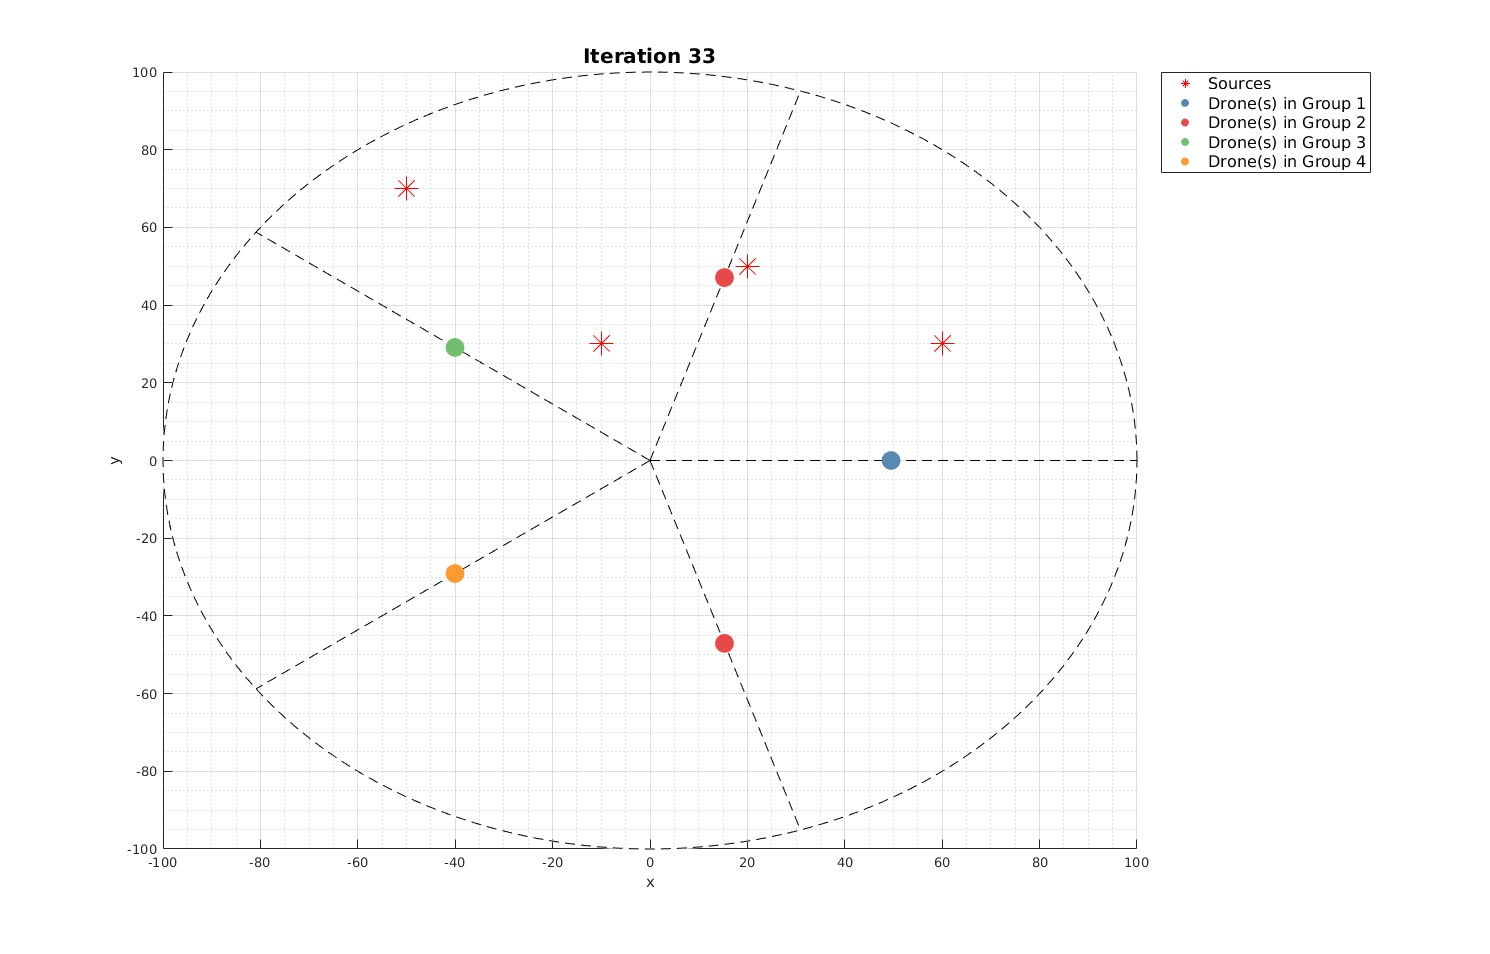
\includegraphics[width=\textwidth]{images/exploration_pattern.jpg} 
%     \caption{Radial exploration pattern for 5 drones at the end of the Exploration Phase.}
%     \label{fig:exploration_pattern}
% \end{figure}

\subsubsection{Exploitation Phase}
This is the most important part of the simulation since it involves
the localization of the victims through the deployment of our modified PSO
algorithm with the PID control, described in Section \ref{sec:PSO+PID}.

\noindent\\
At each $\tau_s$ iteration step until \texttt{n\_iterations},
each $j$-th UAV checks the neighbouring drones with the
\textit{can\_I\_communicate\_with()} function and with a 
positive response they share their exclusion zones with each other
(if they have found a source). The communication radio (\(r_{\text{comm}}\))
is set to 10\,m.

\noindent\\
Then, it calls \textit{check\_if\_in\_exclusion\_zone()}
to verify if it's position is inside the radius of any of the 
saved exclusion zones.
In case of a positive response, the drone is commanded to 
execute the \textit{move\_away\_from\_exclusion()} function. 
Then, its velocity is reset to zero, and its personal 
best position, \texttt{p\_best}, is assigned to a random point 
far from the new location. Additionally, the $\mathbf{gbest}$ 
is reset to \(-\infty\), and the 
drone's \texttt{nss\_best} is also reset to \(-\infty\), 
ensuring the drone restart exploring with a fresh start.
For simplicity reasons, this movement is considered "instantaneous", 
meaning that in the simulation, the drone's journey to the goal is 
not displayed. Instead, in the next iteration, it will already 
be at the designated location. However, the number of 
iterations and the simulation time account for the actual 
time required for the drone to reach the goal at maximum speed.
In case of a negative response, the \textit{evaluate\_nss()} is 
called and the group best ($\mathbf{gbest}$) is updated if the received NSS signal 
is greater than the previous best.

\noindent\\
Subsequently, the \textit{update\_velocity()} method computes the desired 
velocity command for the control loop and the desired position is obtained 
using the standard PSO formula in Eq. \ref{eq:model_position2}.
At each time step $\tau_k$ until the end of the $\Delta$, 
the \textit{update\_state()} function is called and the
boundries are enforced as in \ref{eq:boundary_condition}.
Finally, we can present the complete modified PSO algorithm in 
Algorithm \ref{alg:PSO}.
\SetAlgoBlockMarkers{}{}
\begin{algorithm}
    \DontPrintSemicolon
    \caption{Particle Swarm Optimization for Multi-Source Localization}\label{alg:PSO}
    \KwInitialize{positions of drones to the center of the search space.}\;
    \KwInitialize{\texttt{g\_best\_values}.}\;
    \textbf{Assign} each drone to a group using the function in Algorithm \ref{alg:sort_drones_in_groups}.\;
    \vspace{0.3\baselineskip}
    \DontPrintSemicolon \nonl \textbf{Exploration Phase:}\; \PrintSemicolon
    \textbf{Compute} exploration goals using the function in Algorithm \ref{alg:exploration_goals}\;
    \For{\forcond}{
        \textbf{Move} to goal with \texttt{max\_velocity}\;
    }
    \vspace{0.3\baselineskip}
    \DontPrintSemicolon \nonl \textbf{Exploitation Phase:}\; \PrintSemicolon
    \For{\( \tau_s = 1 \) to \texttt{n\_iterations}}{
        \For{\forcond}{
            \For{\textbf{each} other drone \(l \neq j\)}{
                \If{\textit{can\_I\_communicate\_with()} \textbf{or} \texttt{victim\_found\_flag} = \text{true}}{
                    \textbf{Share} exclusion zones between \(j\) and \(l\)\;
                }
            }
            
            \If{\textit{check\_if\_in\_exclusion\_zone()} = true}{
                \If{\textbf{drone} \(j\) is not alone in its group}{
                    \textbf{Reassign} drone \(j\) to a new group\;
                    \textbf{Initialize} new \texttt{g\_best} and \texttt{nss\_best}\;
                }
                \textbf{Move} away from exclusion zones\;
                \textbf{Reset} personal best \texttt{p\_best}\;
                \textbf{Set} drone \(j\) \texttt{inertia} to 0.5\;
            }
            \Else{
                \textbf{Evaluate} NSS at \(\mathbf{p}_j(\tau_s)\)\;
                \If{\texttt{nss\_value} \( > \) \texttt{nss\_best}}{
                    \textbf{Update} \texttt{p\_best}\;
                }
                \If{\texttt{nss\_value} \( > \) \texttt{g\_best}}{
                    \textbf{Update} \texttt{g\_best\_values}\;
                }
            }
            \textbf{Compute} desired velocity: \textit{update\_velocity()}\;
            \textbf{Apply} persistence of excitation as in Eq.\eqref{eq:persistence_of_excitation}\;
            \textbf{Limit} velocity to \texttt{max\_velocity} as in Eq.\eqref{eq:velocity_clamping}\;
            \textbf{Desired} position: as in Eq.\eqref{eq:model_position2}\;
            \textbf{Set} \texttt{iteration\_duration} to 1\;
            \For{\(\texttt{t} = 0 : \texttt{dt} : \texttt{iteration\_duration}\)}{
                \textbf{Control} dynamics: \textit{update\_state()}\;
                \textbf{Enforce} boundaries on position as in Eq.\eqref{eq:boundary_condition}\;
            }
        }
    }
\end{algorithm}    
Note that the inertia of a drone that has found a source 
is set to zero (\(\omega = 0.5\)), increasing
convergence speed. The final output is the set of best estimates 
\texttt{g\_best\_values}, composed of the best estimated position 
of a source by each group.

\newpage
\section{Results}
\subsection{PID for Trajectory Tracking}

The results of PID control using the full quadrotor dynamics 
model \eqref{eq:final_model},
applied to trajectory tracking during the first positioning 
(exploration) phase of the algorithm, 
are presented in the following figures: 
Figure \ref{fig:pd_traj_comparison} illustrates 
the comparison between the actual and desired trajectory in 3D space, 
showcasing the effectiveness of the control strategy in 
aligning the drone's path with the desired trajectory.

\noindent\\
The desired trajectory chosen for this phase
is designed to a provide smooth and easily controlled movement. 
The \(x\) and \(y\) components of the trajectory follow 
a linear motion at constant maximum velocity \(v_{\text{max}}\). 
Since the drones need to travel on straight lines that 
radially distribute over the horizontal $xy$-plane, we 
define the \texttt{drone\_angle} in Alg. \ref{alg:exploration_goals} as
\(\gamma \) the orientation w.r.t. the $x$-axis of the trajectory.
The altitude is modeled to rise smoothly 
using an exponential function, achieving a desired altitude \(z_d\), 
with a smoothness factor \(k\) controlling the rate of ascent. 
The mathematical expressions for the desired trajectory and 
its derivatives are:
\begin{equation}
\begin{aligned}
\mathbf{x_d}(t) &= 
\begin{bmatrix}
x_d(t) \\ y_d(t) \\ z_d(t)
\end{bmatrix}
=
\begin{bmatrix}
v_{\text{max}} \, t \cos(\gamma) \\
v_{\text{max}} \, t \sin(\gamma) \\
z_d \left(1 - e^{-k t}\right)
\end{bmatrix} \\[10pt]
\mathbf{\dot{x}_d}(t) &= 
\begin{bmatrix}
\dot{x}_d(t) \\ \dot{y}_d(t) \\ \dot{z}_d(t)
\end{bmatrix}
=
\begin{bmatrix}
v_{\text{max}} \cos(\gamma) \\
v_{\text{max}} \sin(\gamma) \\
z_d k e^{-k t}
\end{bmatrix} \\[10pt]
\mathbf{\ddot{x}_d}(t) &= 
\begin{bmatrix}
\ddot{x}_d(t) \\ \ddot{y}_d(t) \\ \ddot{z}_d(t)
\end{bmatrix}
=
\begin{bmatrix}
0 \\
0 \\
-z_d k^2 e^{-k t}
\end{bmatrix}
\end{aligned}
\end{equation}
    
\noindent\\
Figures \ref{fig:pid_x}, \ref{fig:pid_y}, and \ref{fig:pid_z}
provide a detailed breakdown of the trajectory tracking along 
the \(x\), \(y\), and \(z\) axes, respectively. 
These plots highlight the individual tracking performance 
in each dimension and confirm the controller's precision 
in following the desired positions.


\noindent\\
Figure \ref{fig:pid_sim} shows the simulation over time,
providing an overview of the control system's behavior 
during this phase. Additionally, the rotor velocities 
calculated using \eqref{eq:rotor_velocities} are plotted 
in Figure \ref{fig:rotor_velocities}. 

\noindent\\
The results demonstrate
that after an initial overshooting the position controller
is able to follow the desired trajectory.
In particular, altitude control (hovering) is also quite important in our appplication
and it is successful in our results.
Furthermore, the rotor velocities exhibit regular and achievable values,
meaning the actuation inputs can be followed.
These results were obtained under a nominal scenario, 
where wind disturbances or other environmental factors are not considered,
since the primary focus of this work is not on the control robustness.
\begin{figure}
    \centering
    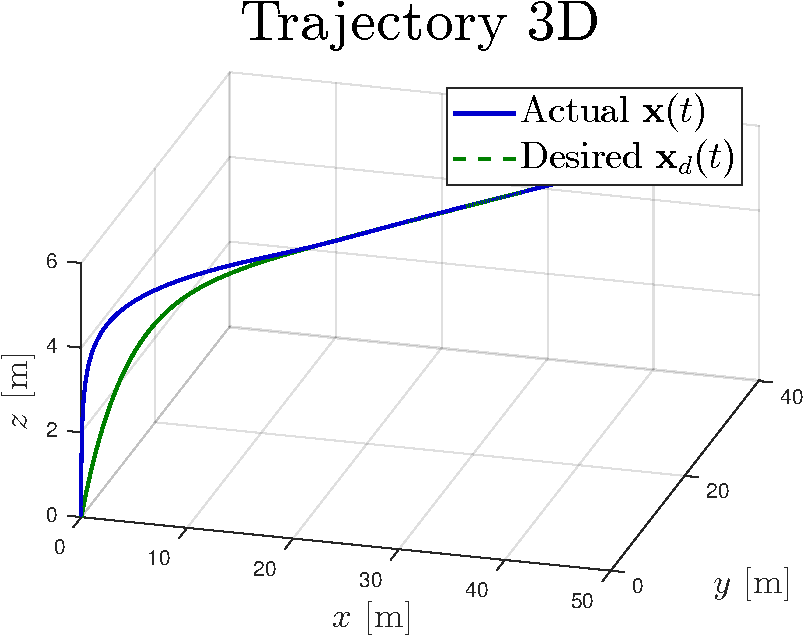
\includegraphics[width=0.8\textwidth]{images/trajectory_comparison.pdf}
    \caption[3D Trajectory Tracking]{Comparison of the actual and desired trajectory in 3D space during the exploration phase.}
    \label{fig:pd_traj_comparison}
\end{figure}

\begin{figure}
    \centering
    \begin{minipage}[b]{0.45\textwidth}
        \centering
        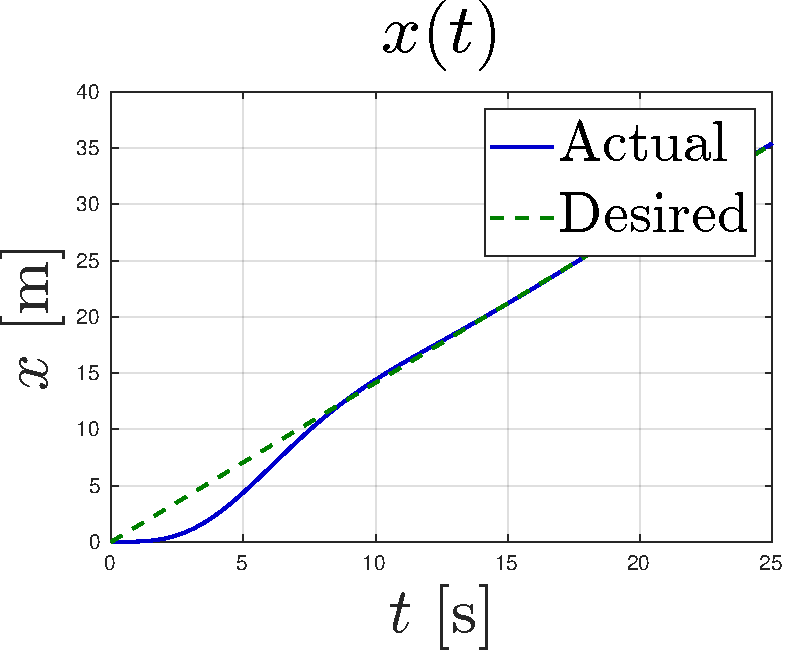
\includegraphics[width=\textwidth]{images/pid_x.pdf}
        \caption[Tracking in X-axis]{Actual and desired $x(t)$.}
        \label{fig:pid_x}
    \end{minipage}
    \begin{minipage}[b]{0.45\textwidth}
        \centering
        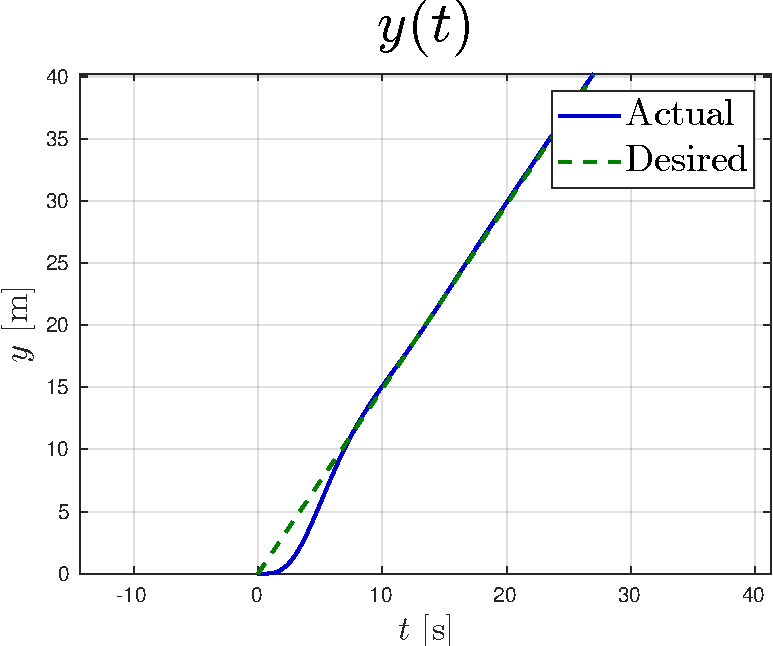
\includegraphics[width=\textwidth]{images/pid_y.pdf}
        \caption[Tracking in Y-axis]{Actual and desired $y(t)$.}
        \label{fig:pid_y}
    \end{minipage}
    \begin{minipage}[b]{0.48\textwidth}
        \vspace{0.4cm}
        \centering
        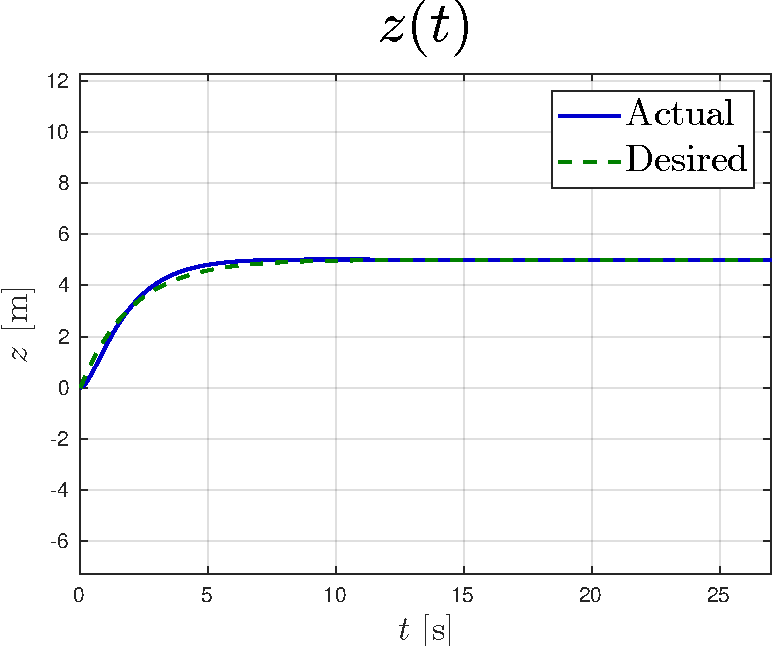
\includegraphics[width=\textwidth]{images/pid_z.pdf}
        \caption[Tracking in Z-axis]{Actual and desired $z(t)$.}
        \label{fig:pid_z}
    \end{minipage}
\end{figure}

\begin{figure}
    \centering
    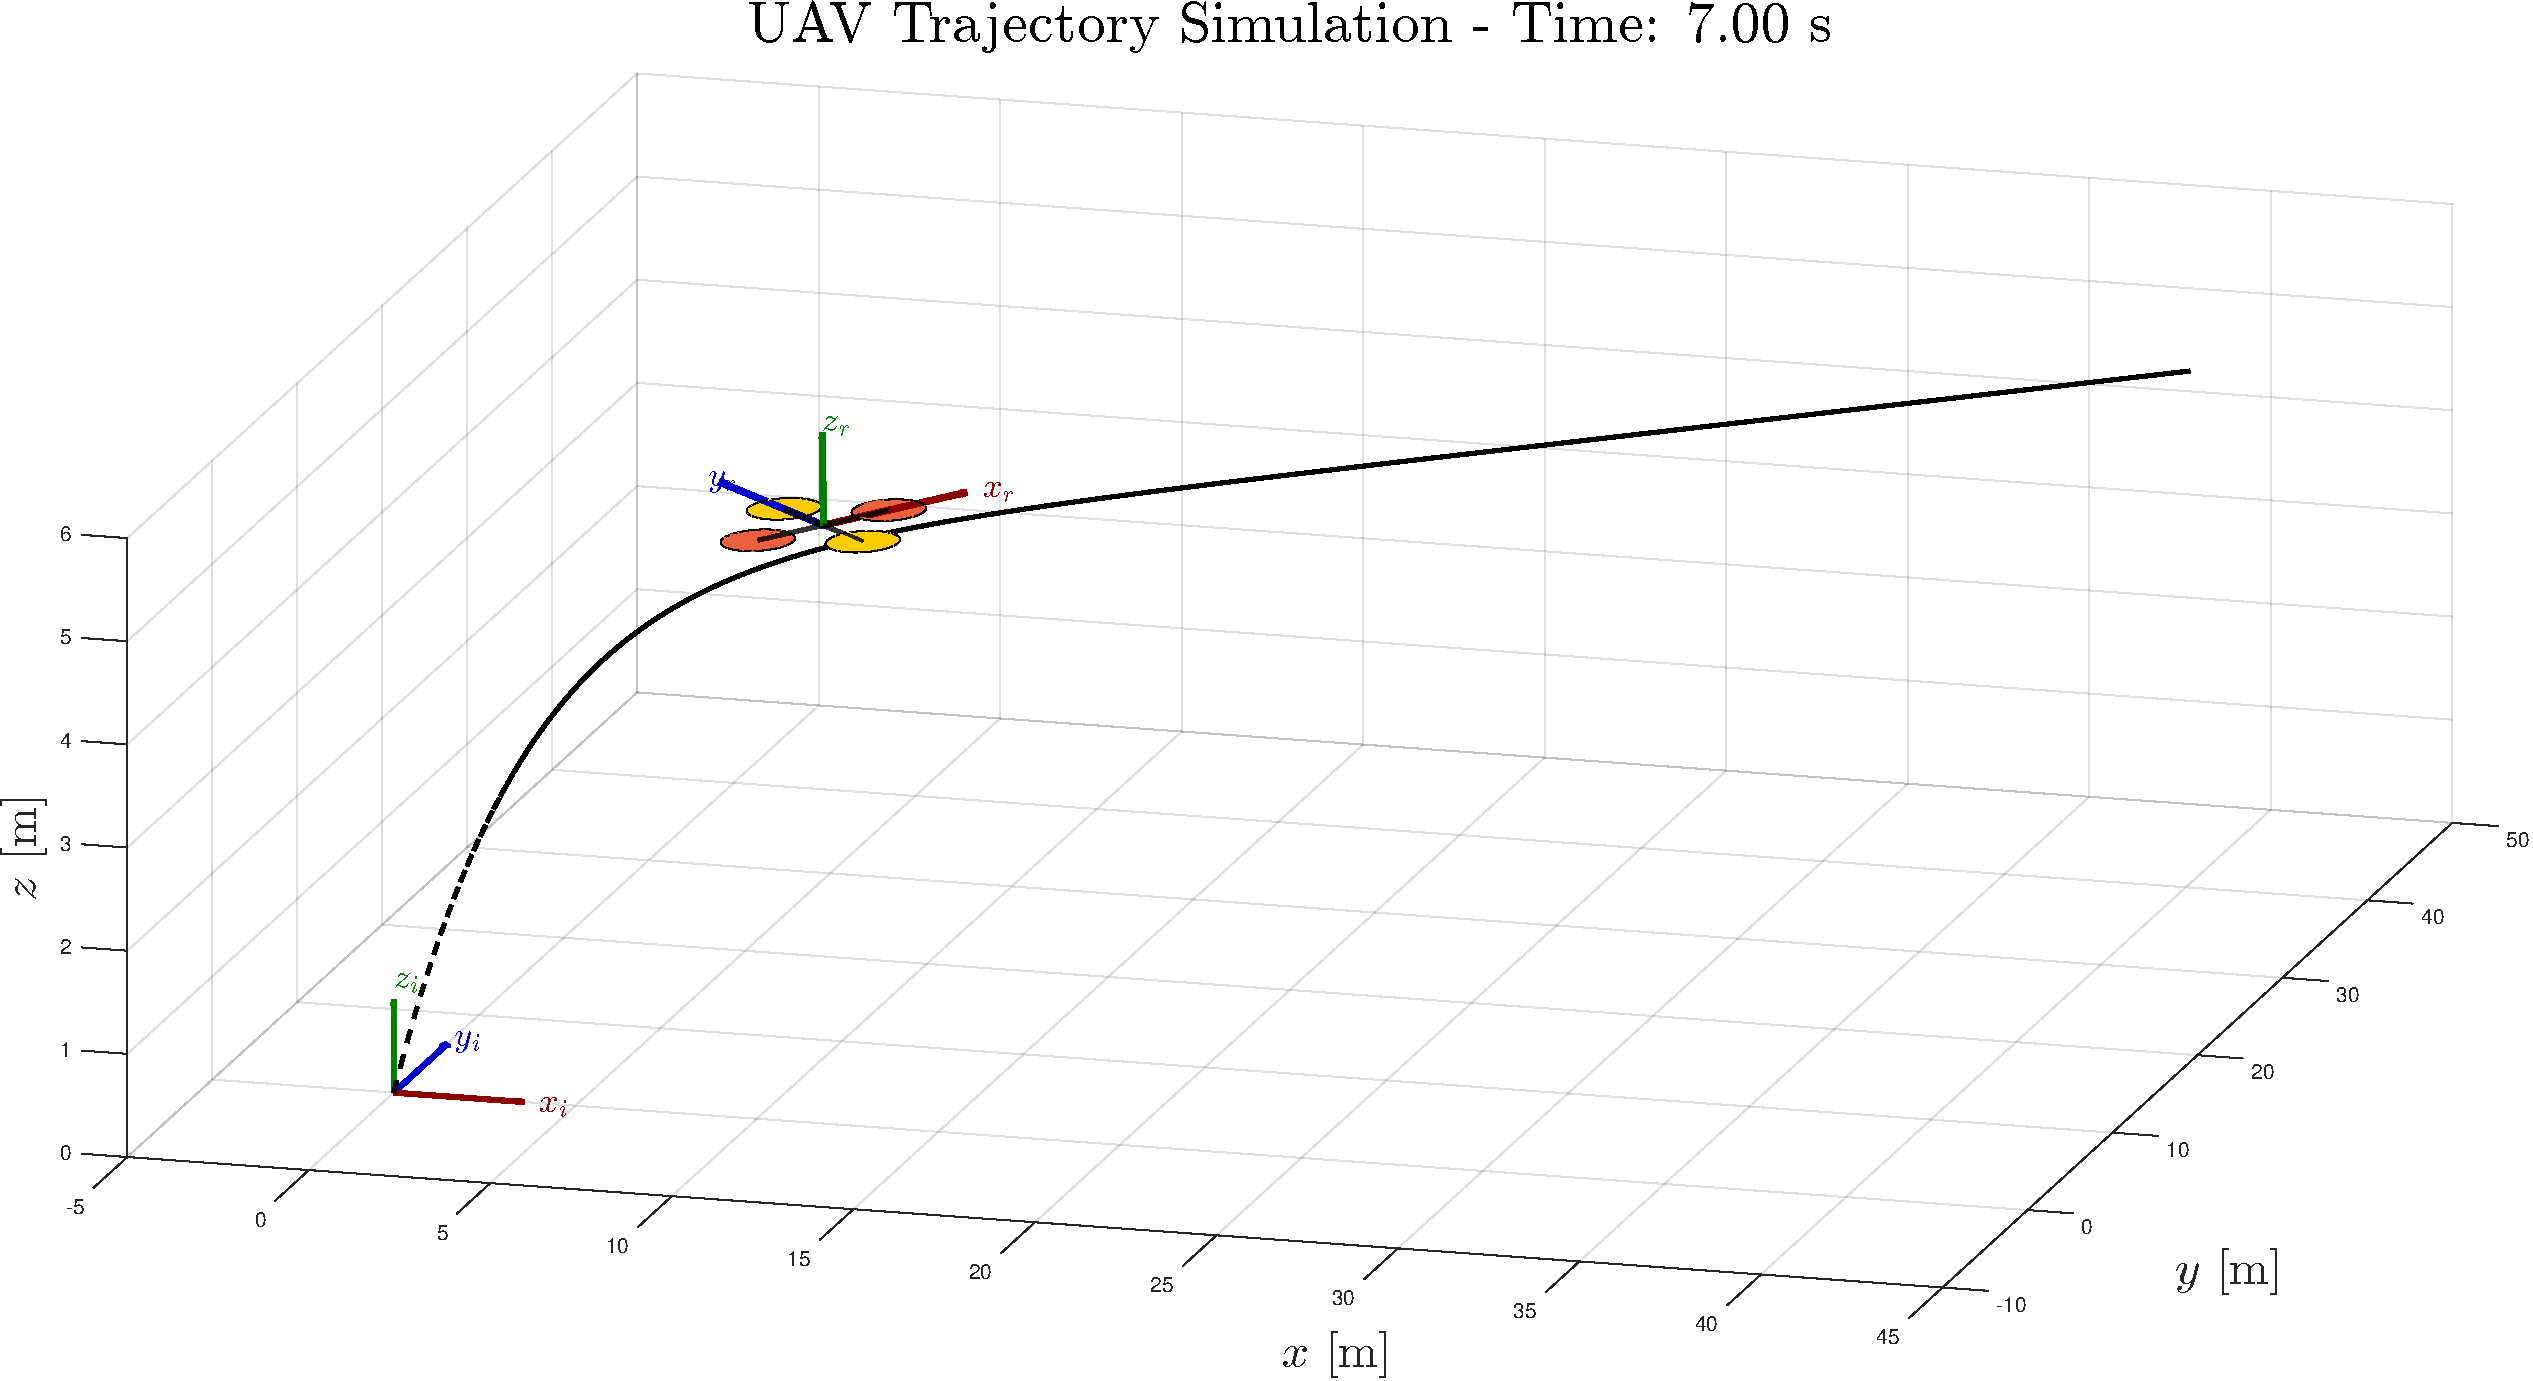
\includegraphics[width=\textwidth]{images/pid_sim.pdf}
    \caption[Simulation Overview]{Time instant during the simulation illustrating the system's dynamic behavior.}
    \label{fig:pid_sim}
\end{figure}

\begin{figure}
    \centering
    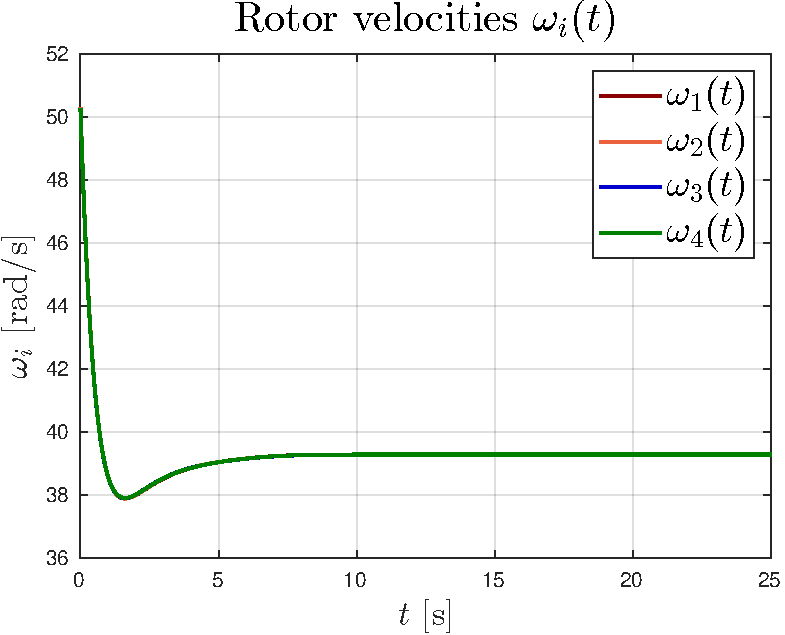
\includegraphics[width=0.7\textwidth]{images/rotor_velocities.pdf}
    \caption[Rotor Velocities]{Rotor velocities over time as calculated using \eqref{eq:rotor_velocities}, the actuation required for trajectory tracking.}
    \label{fig:rotor_velocities}
\end{figure}

\newpage
\subsection{PSO wih Control}
In the context of search and rescue (S\&R) missions, the number of available 
UAVs is typically limited (ranging from 1 to 10 \cite{PSO_original}), and 
the search area 
usually spans only a few thousand square meters.
In order to have faster simulations and more constrained 
values we limit the search space 
to the hundreds of meters.
However, the algorithm is scalable to bigger distances while mantaining the same
performances by incrementing the drones' speed, or enhancing the capabilities
of the ARTVA receiver, which is usually limited to our chosen limits.

Each drone in the PSO control integrated framework is 
initialized with the hyperparameters described in the previous sections. 
The drones start their search with an initial position at the 
center of the search space, defined as \([0, 0]\). 
Their initial velocities are randomized using the velocity randomness
factor capped at a maximum velocity of \(2 \, \text{m/s}\) 
to prevent overshooting targets. The search space is constrained within bounds 
of \([-80, 80] \, \text{m}\) for both the \(x\) and \(y\) directions.

Each drone's best-known position ($\mathbf{pbest}$) is initialized 
to its starting position, while its best NSS
value is set to \(-\infty\), ensuring that any detected signal improves 
its current state. The drones operate with an inertia weight of \(1.05\), 
balancing exploration and exploitation during the optimization process. 

The drones are grouped based on a variable group index, and 
each group best-known position ($\mathbf{gbest}$) is also 
initialized to \(-\infty\).
reagarding the orientation and UAVs dynamics, the roll, pitch, and yaw angles
are initialized to \([0, 0, 0]\).
The initial velocity during the second phase of the algorithm is the same
of the arriving velocity at the goal of the first phase.
These parameters collectively define the initial state and behavior of the 
drones in the PSO framework.
In the following sections we report the results relative to 3 different 
scenarios regarding the number of drones employed and the positions of the victims
in space, under nominal conditions both for the ARTVA signal and the PID controller.

\subsection{Case 1}
In the first case, the PSO algorithm needs to locate four sources positioned 
at \([20, 50] \, \text{m}\), \([-50, 70] \, \text{m}\), \([60, 30] \, \text{m}\), 
and \([-10, 30] \, \text{m}\), 
randomly distributed across the search space.

\noindent\\
The time it took for the swarm to find the victims was 292 seconds (\(\sim 4.9\) minutes),
during which the drones successfully converged on the sources, 
achieving precise estimates with an average error of \(0.09 \, \text{m}\). The estimate for the first source was 
just \(0.025 \, \text{m}\) away, while the second, third, and fourth sources were 
located with errors of \(0.287 \, \text{m}\), \(0.013 \, \text{m}\), and \(0.053 \, \text{m}\), respectively.

\noindent\\
In Figure~\ref{fig:case1} we can see  
the sources' locations and the drones' trajectories duing the PSO 
optimization process, from which is evident that the exclusion zone mechanism
worked in favour of drones 3 and 4 in successfully locating a source.

\begin{figure}
    \centering
    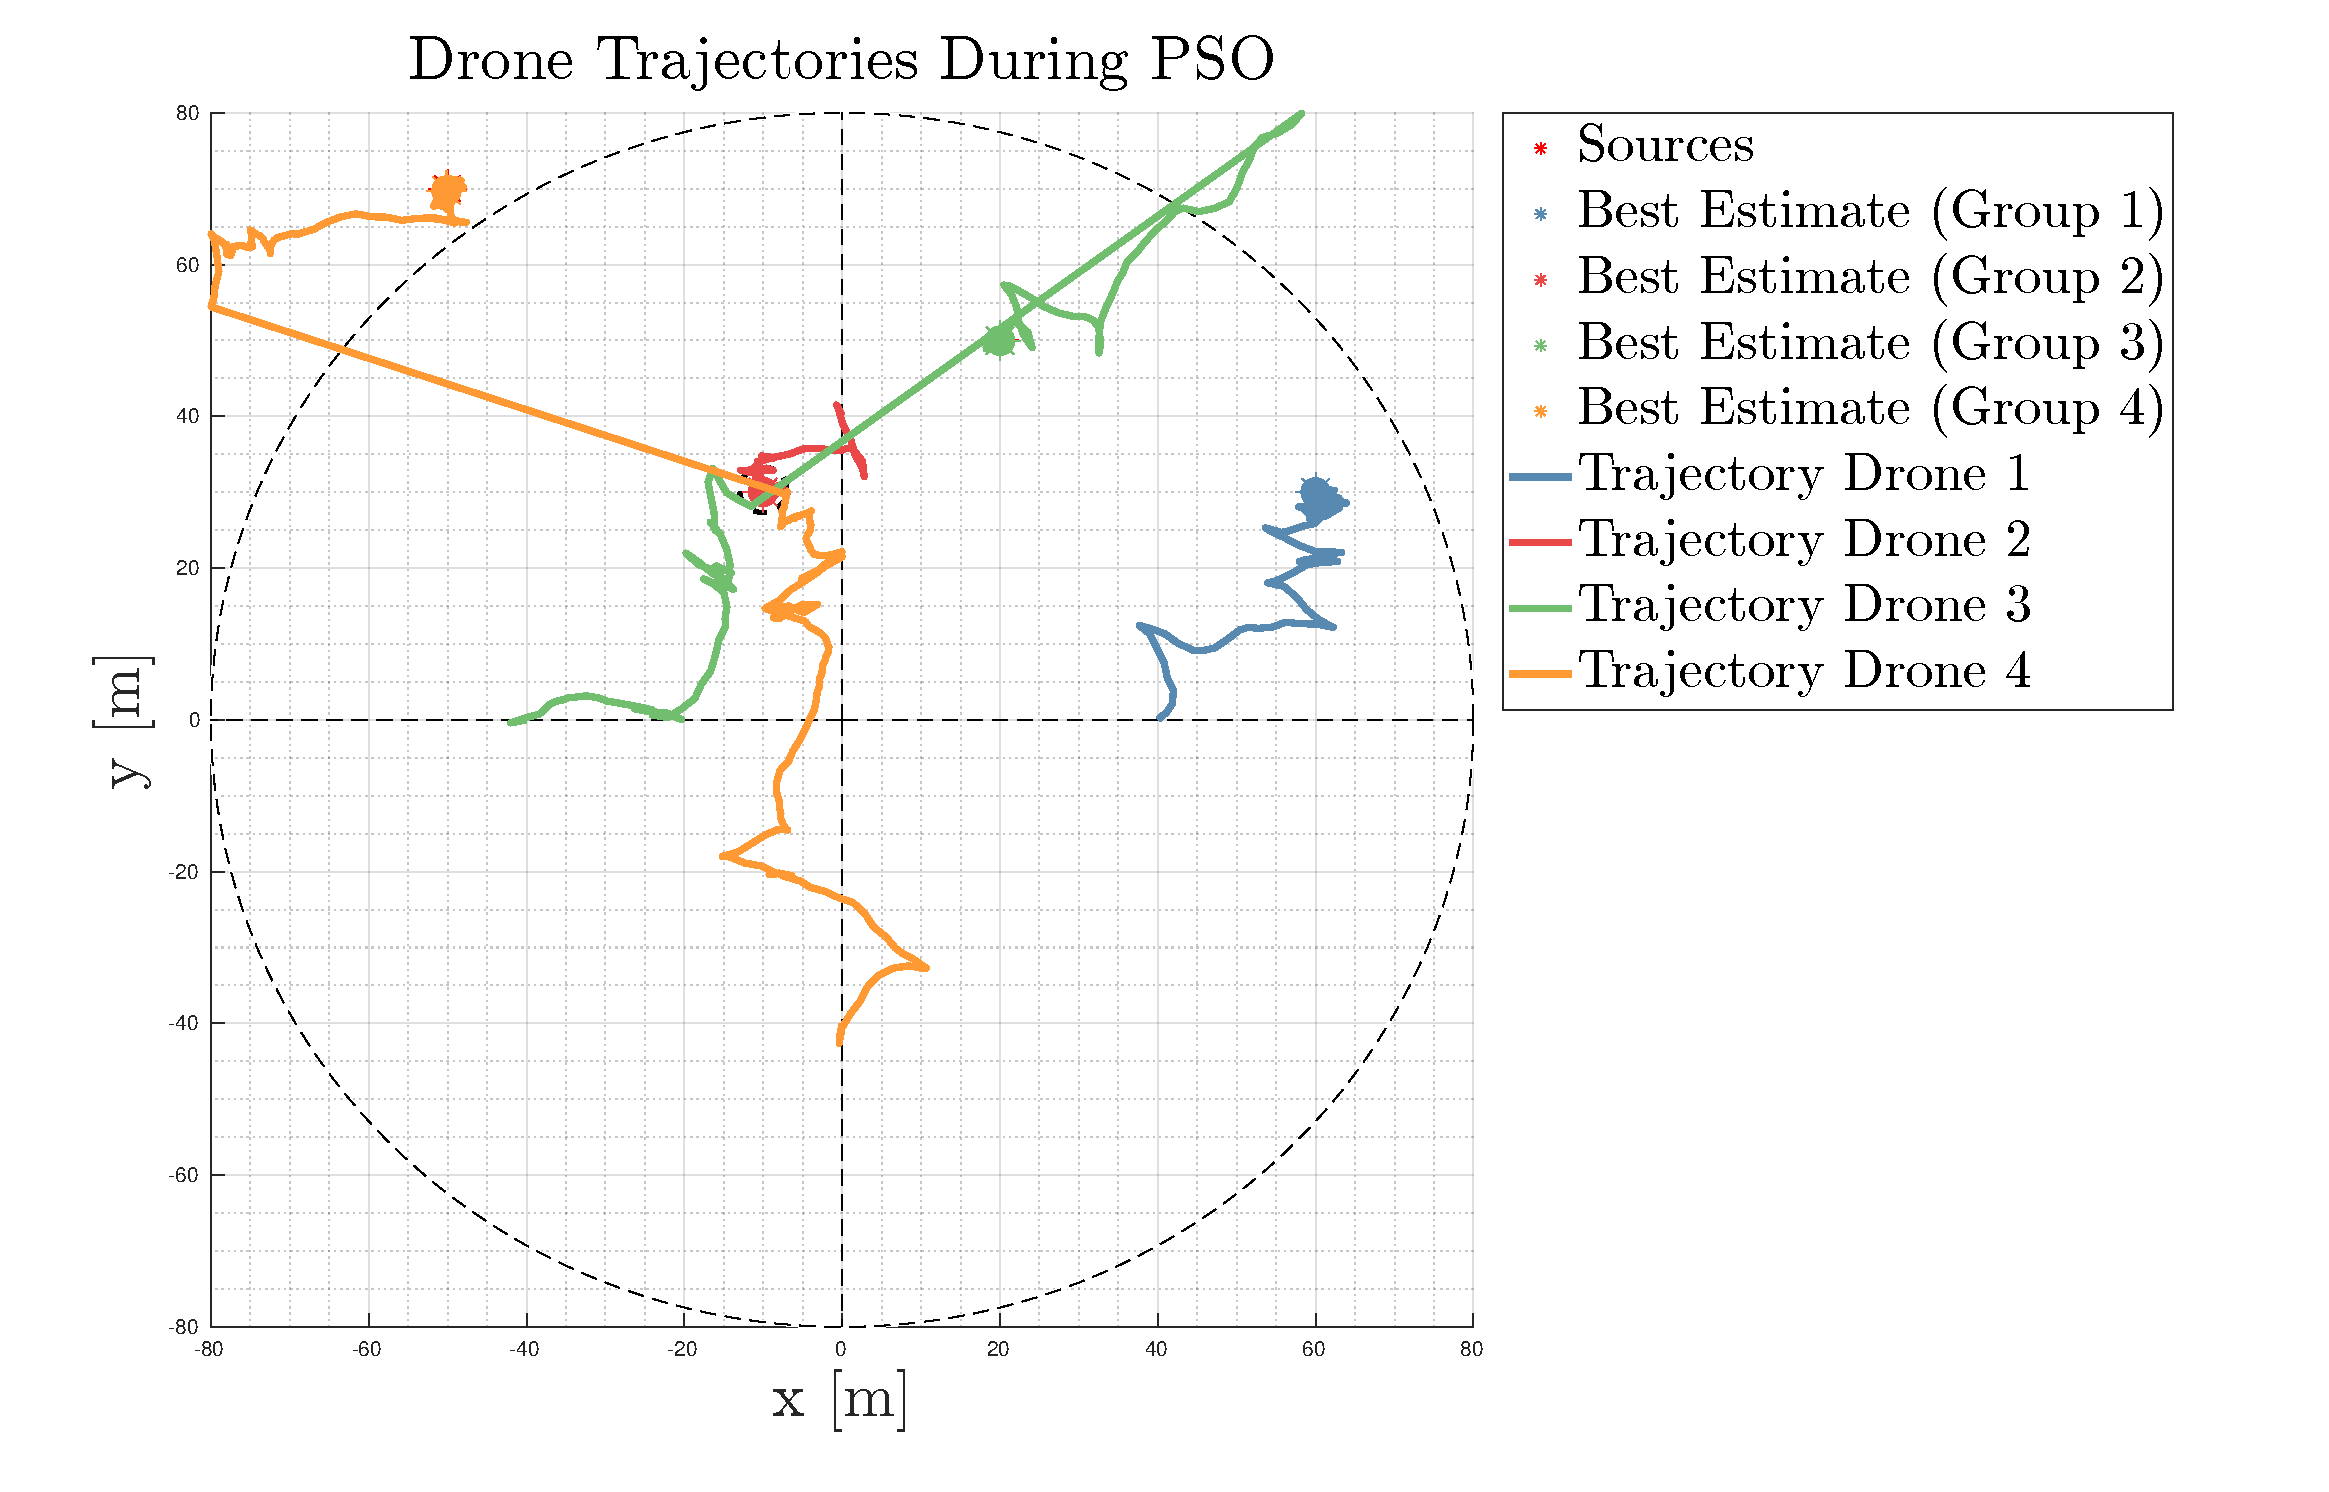
\includegraphics[width=1.06\textwidth]{images/case_1.pdf}
    \caption[PSO Case 1]{Results and Trajectories in Case 1.}
    \label{fig:case1}
\end{figure}

\subsection{Case 2}
In the second case, the PSO algorithm is again tasked with locating four 
sources positioned at \([-70, -70] \, \text{m}\), \([70, 70] \, \text{m}\), \([-70, 70] \, \text{m}\), and \([70, -70] \, \text{m}\), 
distributed very far apart across the search space.

\noindent\\
The time it took for the swarm to locate the sources was 336 seconds (\(\sim 5.6\) minutes). 
During this time, 
the drones successfully converged on the sources, achieving an average error of \(0.10 \, \text{m}\). 
The estimates for all the sources were: the first source was \(0.16 \, \text{m}\) away, 
the second was \(0.002 \, \text{m}\) away, the third was \(0.001 \, \text{m}\) away, 
and the fourth was \(0.233 \, \text{m}\). 

\noindent\\
In Figure~\ref{fig:case2}, the sources' locations and the drones' 
trajectories during the PSO optimization process are depicted. 
This case is one of the most complicated since the sources are near
the borders of the search space and therefore
the signal they send are less strong.
\noindent\\
To evaluate the impact of increasing the number of drones, a second simulation 
was conducted by adding an additional drone to the swarm. 
Naturally, we see improved performance in the total time
needed by the UAVs to find all victims, which was just 137 seconds (\(\sim 2.3\) minutes).
The average error across all sources slightly increased to \(0.26 \, \text{m}\),
due to the very high time reduction which did not consent the drones
to converge towards more precise positions. 
Instead, the time improvement was due to some drones 
having a better trajectory during the exploration phase, which brougth 
them nearer the sources.
Figure~\ref{fig:case2more} illustrates the results of this improved configuration. 

\begin{figure}
    \centering
    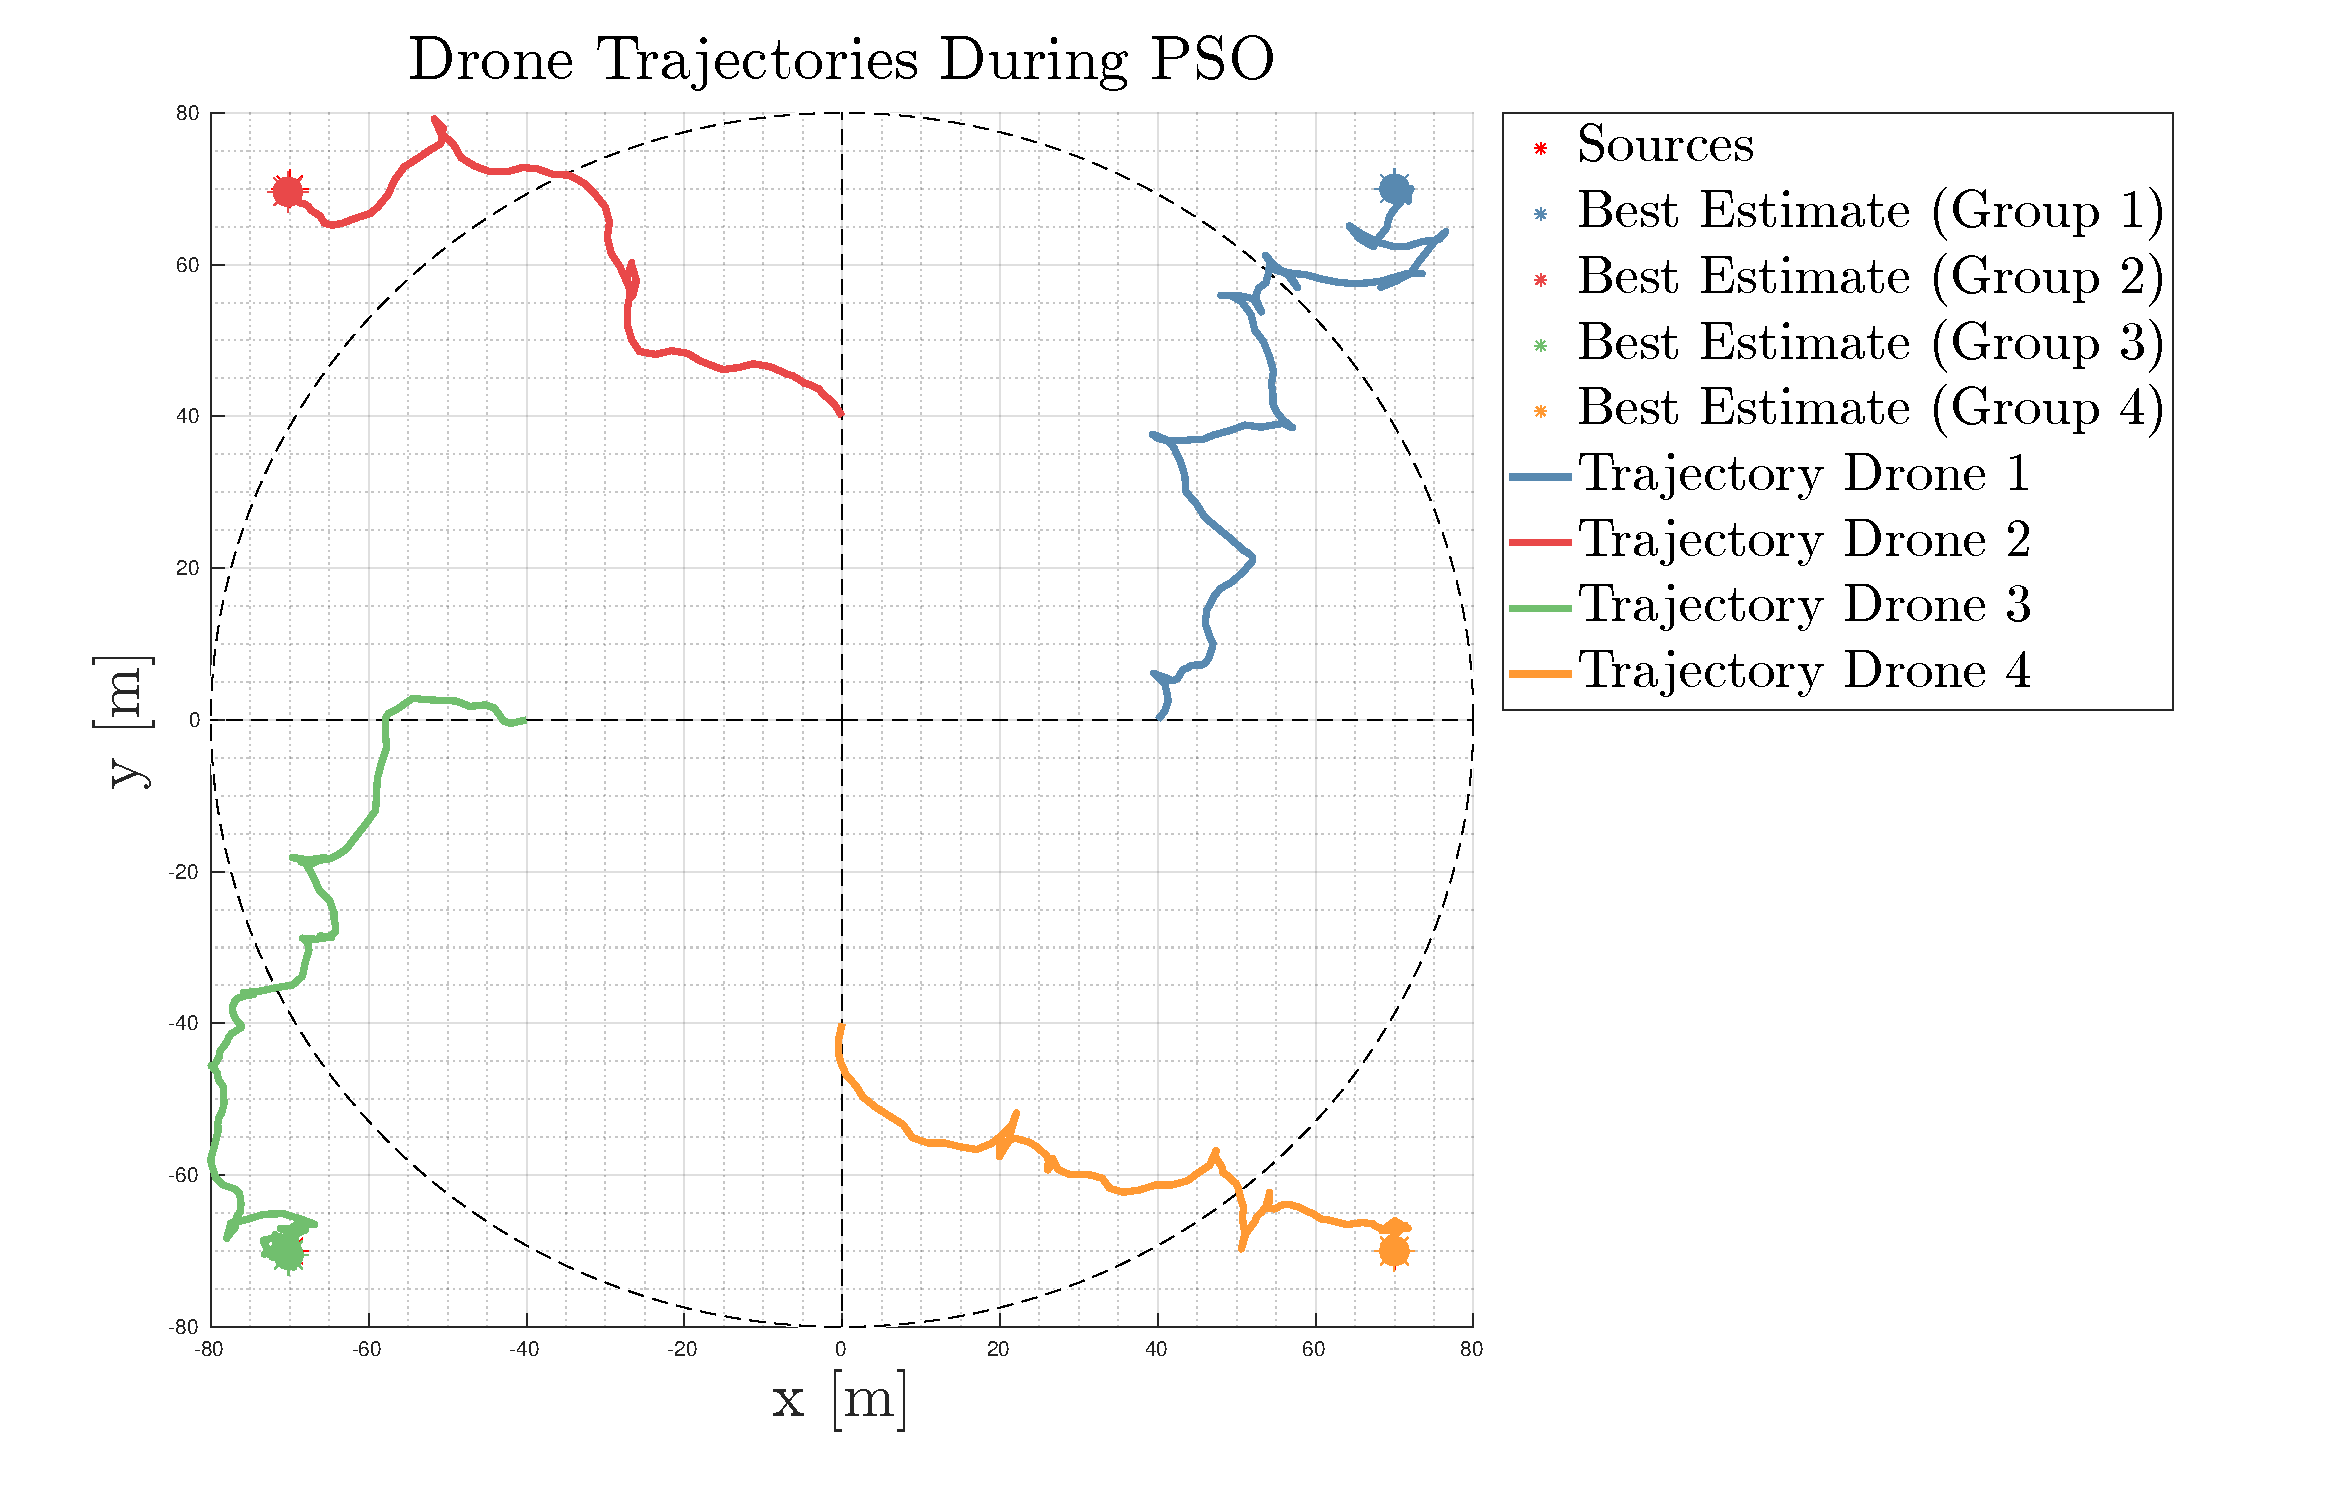
\includegraphics[width=1.06\textwidth]{images/case_2.pdf}
    \caption[PSO Case 2]{Results and Trajectories in Case 2.}
    \label{fig:case2}
\end{figure}
\begin{figure}[H]
    \centering
    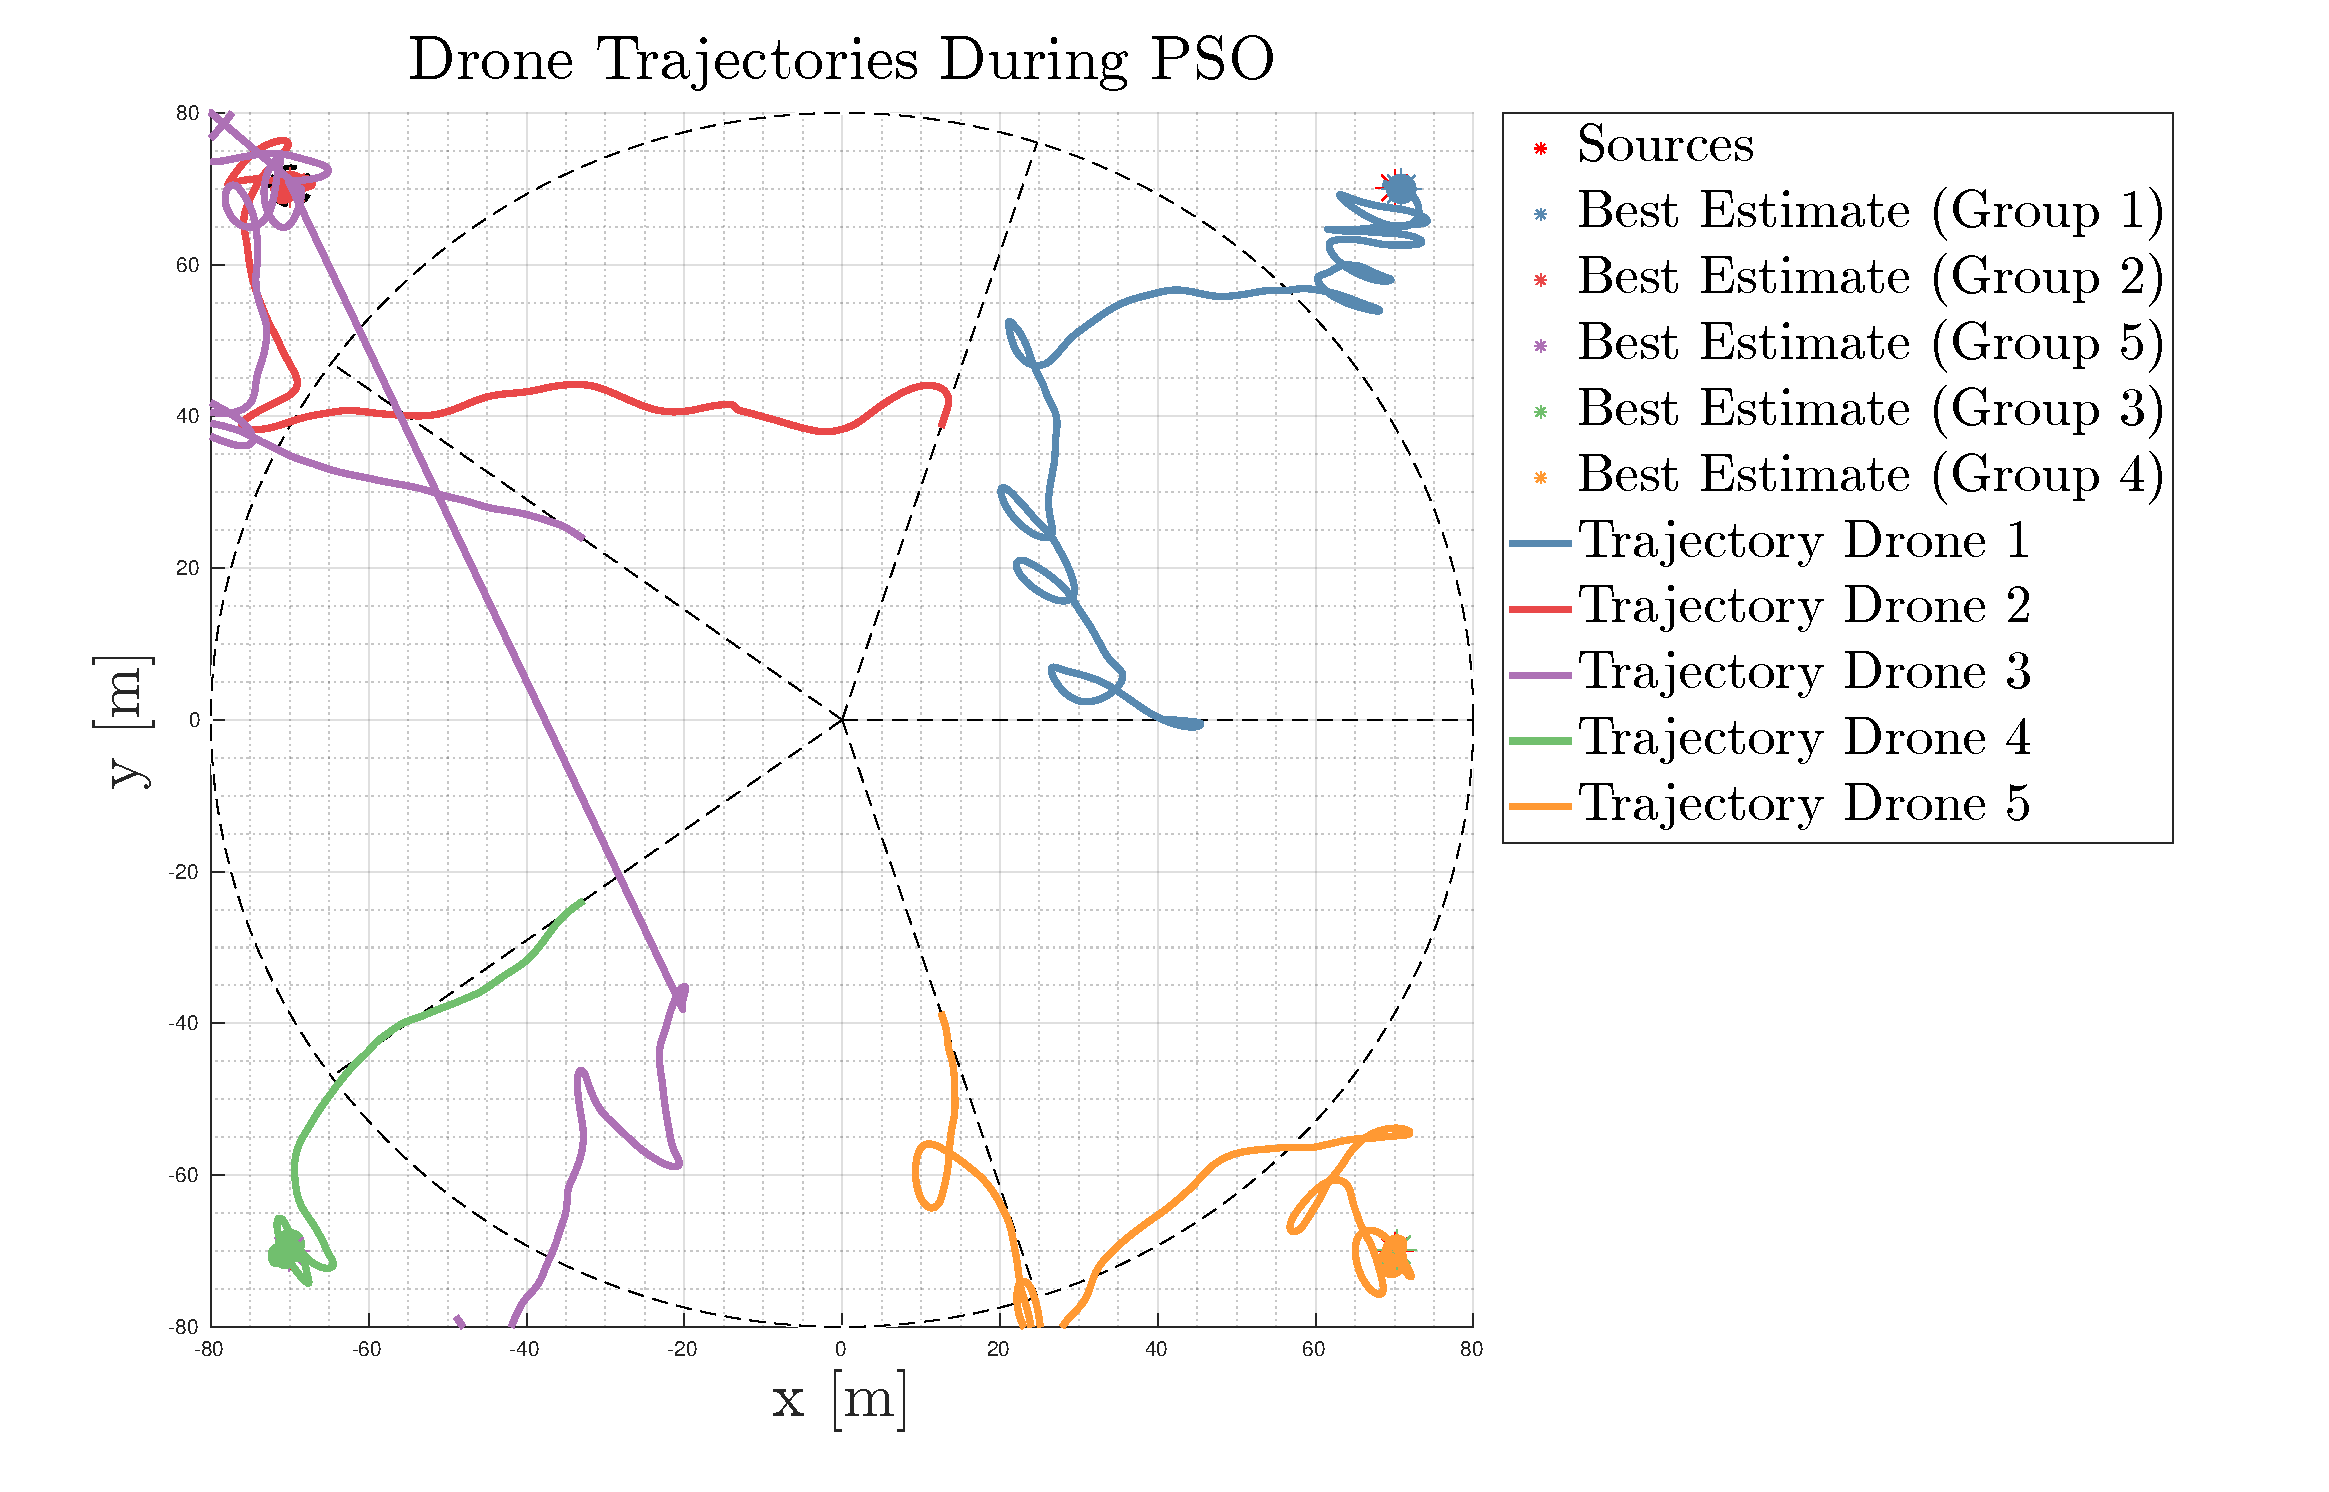
\includegraphics[width=1.06\textwidth]{images/case_2_more.pdf}
    \caption[PSO Case 2]{Results and Trajectories in Case 2 with an additional drone.}
    \label{fig:case2more}
\end{figure}

\subsection{Case 3}
In the third case, the PSO algorithm faces a challenging scenario where 
the four sources are positioned very close to each other, only \(6 \, \text{m}\) apart, 
at \([20, 50] \, \text{m}\), \([26, 50] \, \text{m}\), \([20, 56] \, \text{m}\), and \([26, 56] \, \text{m}\). 
This situation is particularly difficult for the algorithm due to 
the fact that we have an exclusion zone radius of \(3 \, \text{m}\) and 
whenever one drone gets inside the exlusion zone of another
it has to go \(120 \, \text{m}\) away.
Therefore, when three drones have found their sources, the fourth has only a few
possible directions to reach the fourth source.

\noindent\\
Initially, with four drones, the algorithm fails to reliably 
locate all sources within the 500 seconds allocated for the simulation,
as seen in Figure~\ref{fig:case3fail}. 
While increasing the simulation time could potentially improve performance, 
this approach is unsuitable for our time-sensitive application, where
avalanche victims have a real chance of surviving only within 15 minutes
after the time of the accident.

\noindent\\
To address this issue, an additional drone is introduced, increasing the 
swarm size to five drones. Now, the algorithm successfully 
locates all sources in 293 seconds (approximately \(4.9\) minutes). 
The estimates for the sources are: the first source was \(0.245 \, \text{m}\) away, 
the second was \(0.32 \, \text{m}\) away, the third was \(0.265 \, \text{m}\) away, and the 
fourth was \(0.12 \, \text{m}\) away. The total error for all valid estimates was 
reduced to \(0.24 \, \text{m}\), demonstrating the effectiveness of increasing the 
swarm size in challenging scenarios.
In Figure~\ref{fig:case3}, the addition of a fifth drone and the subsequent 
success in the localization can bee seen clearly.

\begin{figure}
    \centering
    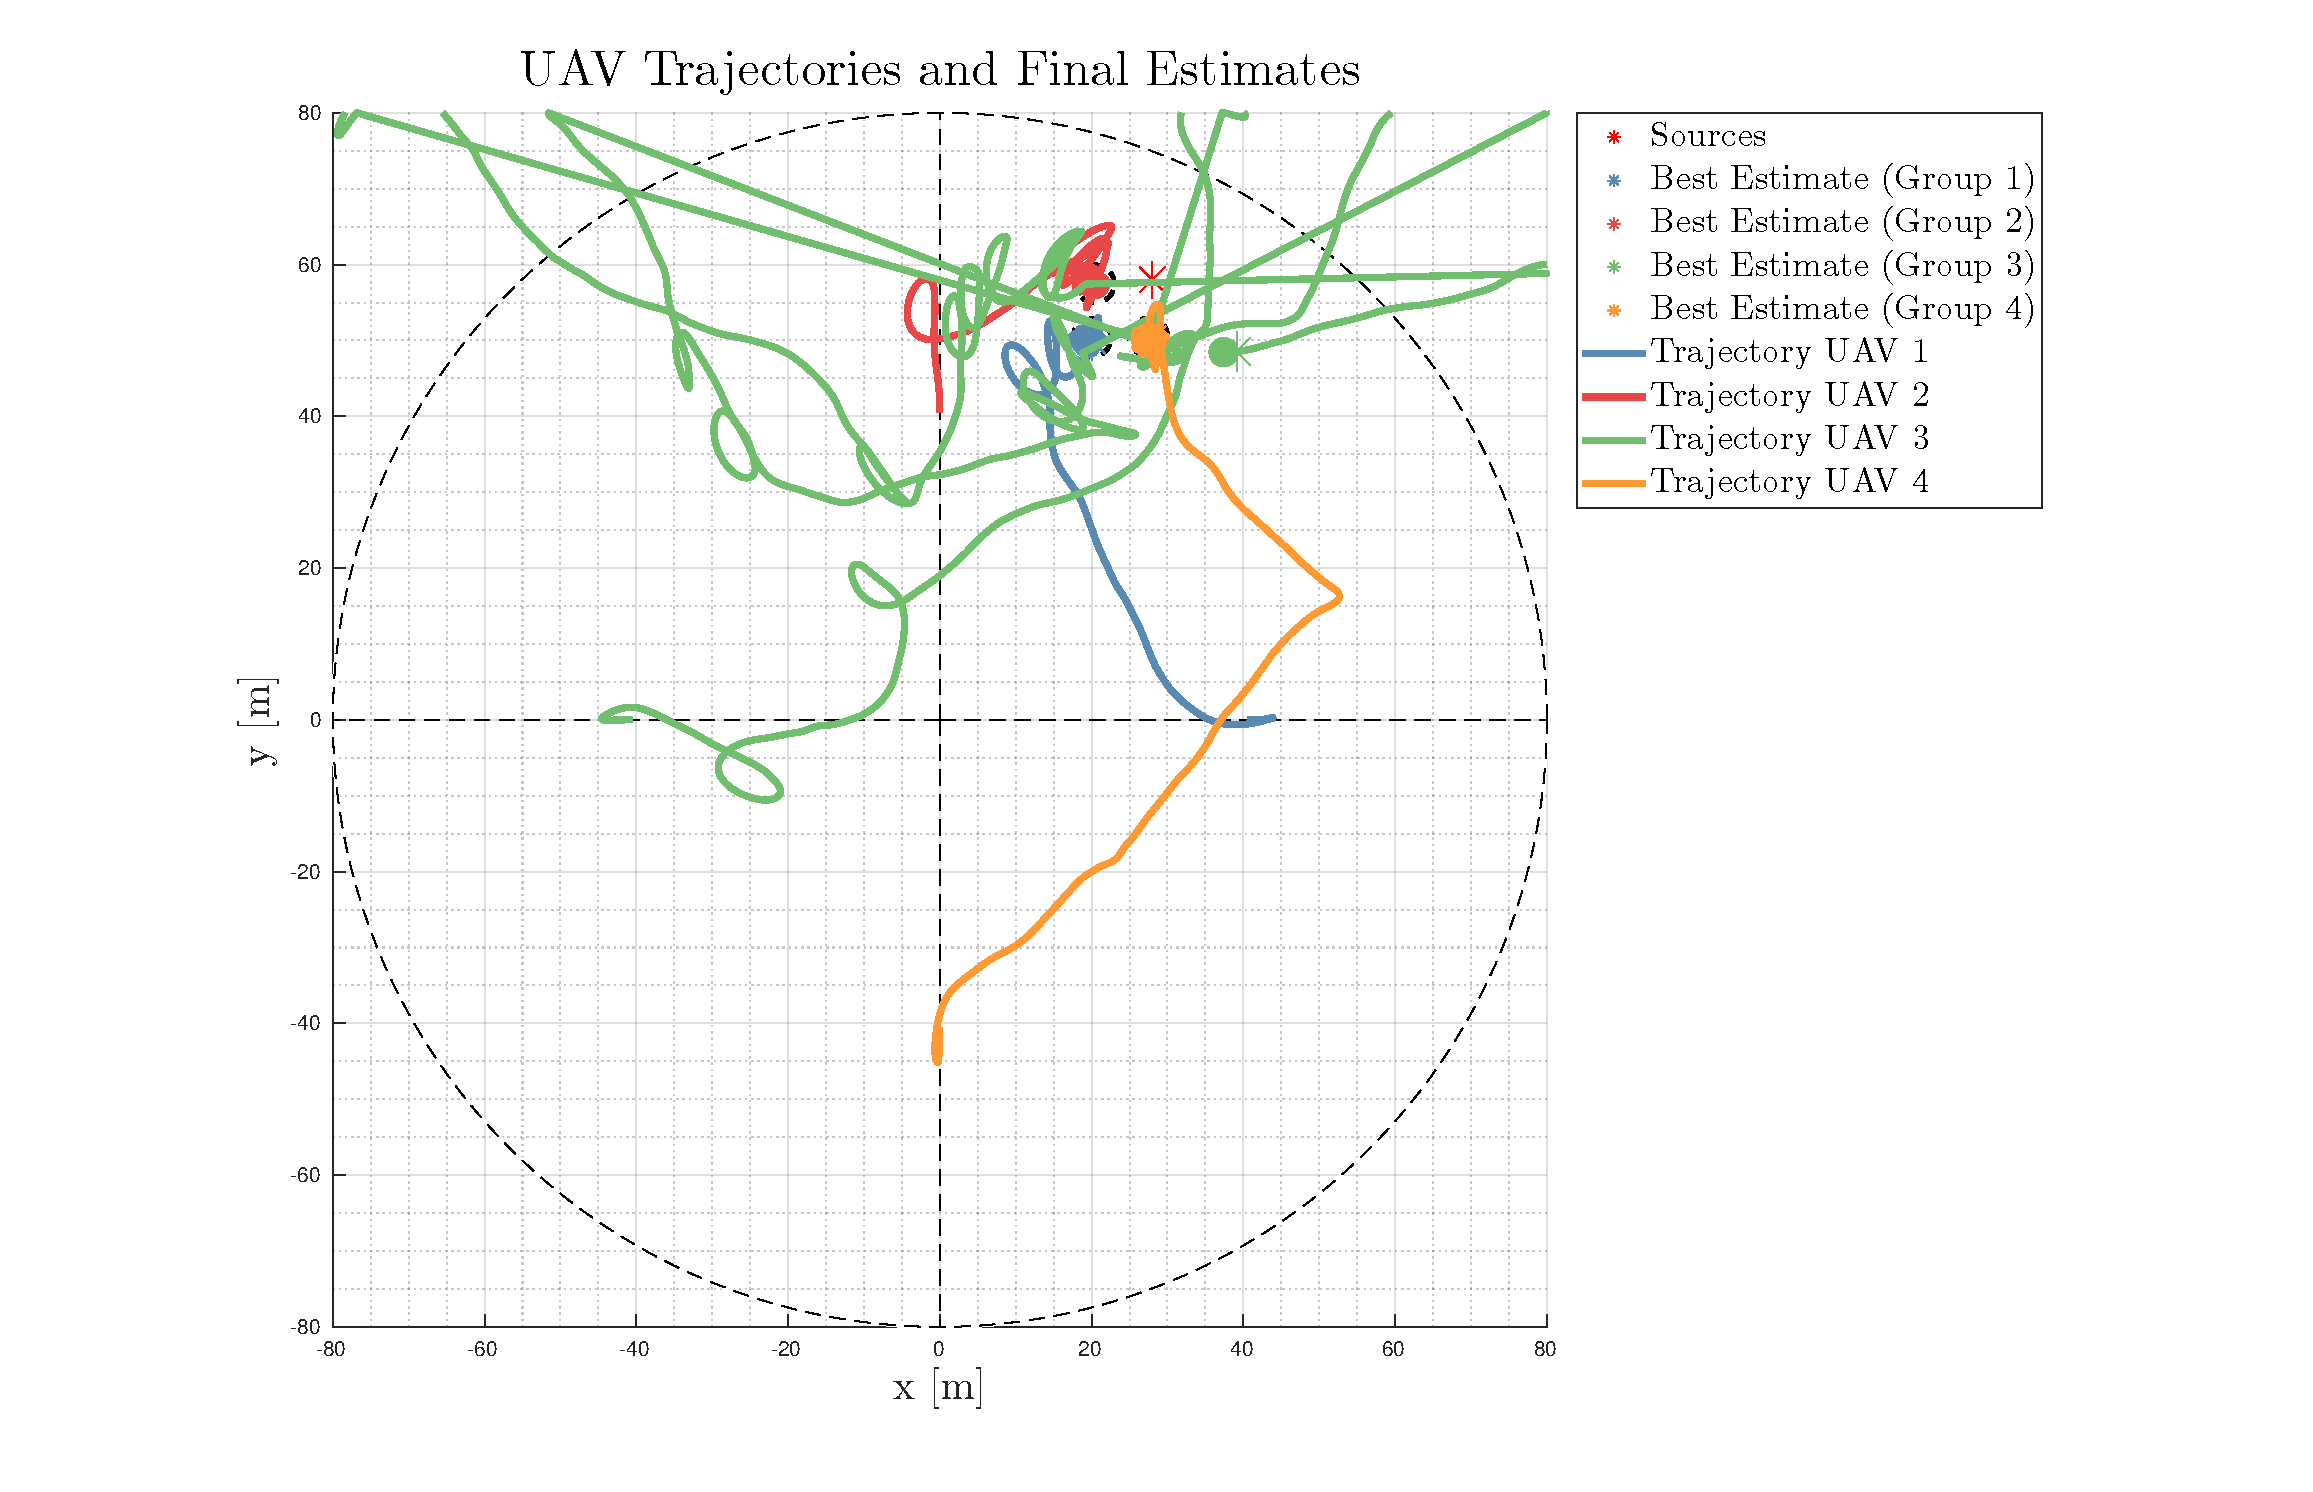
\includegraphics[width=1.06\textwidth]{images/case_3_fail.pdf}
    \caption[PSO Case 3]{Results and Trajectories in Case 3 with fail.}
    \label{fig:case3fail}
\end{figure}



\begin{figure}
    \centering
    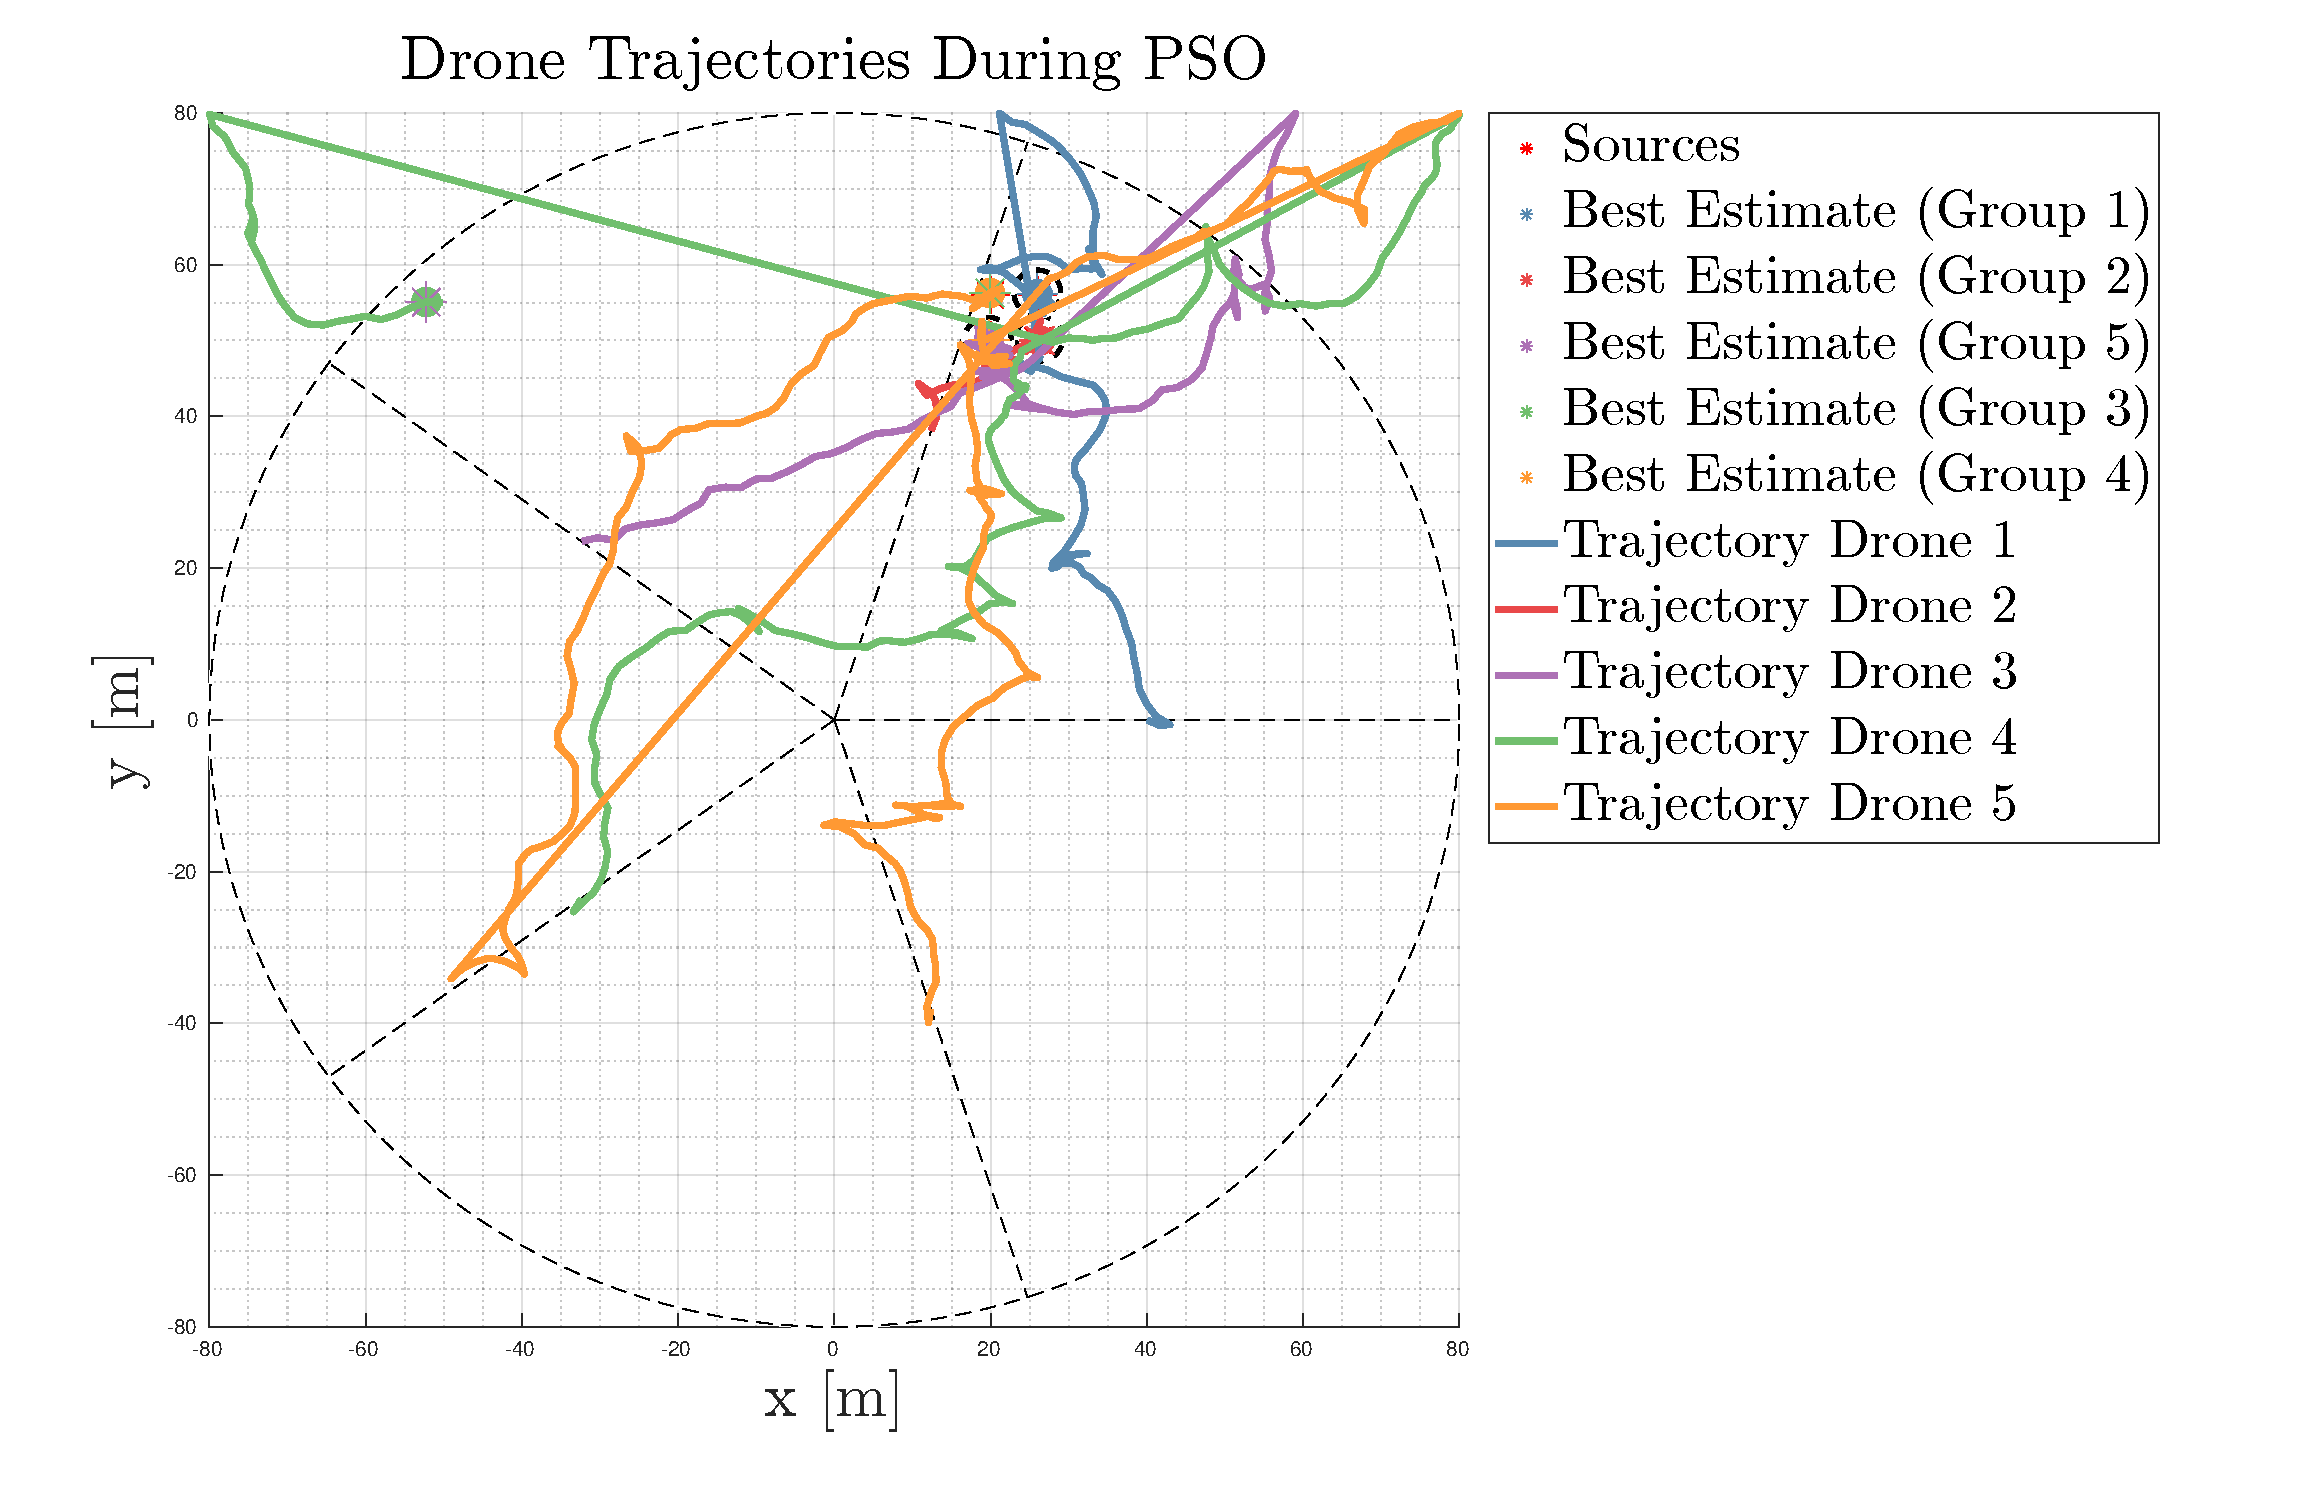
\includegraphics[width=1.06\textwidth]{images/case_3.pdf}
    \caption[PSO Case 3]{Results and UAVs Trajectories in Case 3 with an additional drone.}
    \label{fig:case3}
\end{figure}


\section{Conclusions}
%RILEGGERE LE CONCLUSIONI
In this work, we modify the PSO algorithm to address the challenging
task of multi-source localization using a decentralized swarm of UAVs.
The results show that, in general, the algorithm produces reliable
performance with precise estimates and fast convergence times, even in
complex configurations. However, as an inherently heuristic approach,
the PSO is not guaranteed to always converge, and certain situations
highlight its potential drawbacks.

\noindent\\
One of the main challenges we face is overcoming the superposition in
signal strength from multiple sources or victims. This is our primary
focus, as it inherently complicates the identification of individual
sources. To address this issue, we implement a strategy (the PSO) that
allows the swarm to localize multiple sources based on the aggregated
signal, effectively bypassing the need to separate and identify
individual ones. While this approach proves successful in enabling the
swarm to locate sources in challenging scenarios, it introduces a
trade-off: the certainty of finding a source is reduced because the PSO
heuristic approach relies on some degree of randomness and the exclusion
zone mechanism.

\noindent\\
Another notable drawback is that the algorithm occasionally fails in
scenarios where drones are repeatedly attracted to the same sources,
preventing effective exploration of the search space. This limitation
prevents the swarm's ability to identify and reach faraway
sources, when near others. This behavior is an intrinsic limitation of 
the problem. Additionally, when sources
are positioned too closely together, as demonstrated in Case 3, the
algorithm struggles to differentiate between them, resulting in reduced
accuracy unless additional drones are introduced to improve coverage.

\noindent\\
One potential enhancement in our algorithm is the emplyment of an adaptive mechanisms 
for tuning the PSO parameters, such as inertia weight 
which could dynamically adjust based on the swarm's progress or environmental 
conditions, improving convergence speed and accuracy.
In addition, investigating hybrid optimization methods that combine 
the PSO with local search or other heuristic approaches could provide a more 
comprehensive solution for complex multi-source localization tasks.

\noindent\\
On the other hand, the algorithm's strengths lie in its adaptability and
the benefits of a decentralized approach. The exclusion zone mechanism
enables the swarm to dynamically adjust its search strategy based on the
locations of previously detected sources, promoting faster convergence
and improved accuracy. This adaptability is especially valuable in
multi-source localization problems, where the location of all different
sources rapdly is crucial.
Furthermore, our work also introduces aother novel aspect: 
the implementation of the PSO algorithm to provide control command velocities 
to the drones in real time, integrating the PSO in the control
loop.

\noindent\\
The decentralized nature of our approach offers further advantages. By
removing the reliance on a central computation unit, the system becomes
more robust to communication noise and failures. This autonomy allows
the drones to operate effectively under challenging conditions, such as
mountainous terrain or adverse weather, where communication may be
intermittent or delayed. While decentralization may lead to slightly
slower convergence and higher estimation errors due to partial
information exchange, it remains an effective solution in scenarios
where centralized coordination is impractical or resource-intensive.

\noindent\\
In conclusion, our implementation demonstrates that while the modified PSO
algorithm encounters limitations in specific cases, it provides a
powerful and flexible tool for decentralized multi-source localization.
By addressing the challenge of signal overlap, our algorithm proves to be
both effective and efficient in complex conditions and environment associated
with avalanche victims locatization.